\documentclass[10pt,leqno, oneside]{book}
\usepackage{amsmath,amssymb,amsfonts} % Typical maths resource packages
\usepackage{graphics}                 % Packages to allow inclusion of graphics
\usepackage{color}                    % For creating coloured text and background
\usepackage{hyperref}                 % For creating hyperlinks in cross references
\usepackage{multirow}
\usepackage{bm}
\usepackage{enumitem}
\parindent 0.5cm
\parskip 0cm
\topmargin 0cm 
\oddsidemargin 0cm
\evensidemargin 0cm
\textwidth 16cm
\textheight 21cm
\title{LBNL-AMO-MCTDHF \\
~ \\ %is \\
~ \\
\Large 
Multiconfiguration Time-Dependent Hartree Fock \\
~ \\
for ultrafast electronic and nonadiabatic nuclear dynamics \\
~ \\
of atoms and molecules in intense laser fields \\
~ \\
~ \\
~ \\
Version 1.20 \\
~ \\
%Atomic / Diatomic Rovibronic / Polyatomic Vibronic \\
Atomic / Diatomic Vibronic / Polyatomic Fixed-Nuclei \\
~ \\
%\begin{figure}[!h]
\begin{center}
\resizebox{0.5\textwidth}{!}{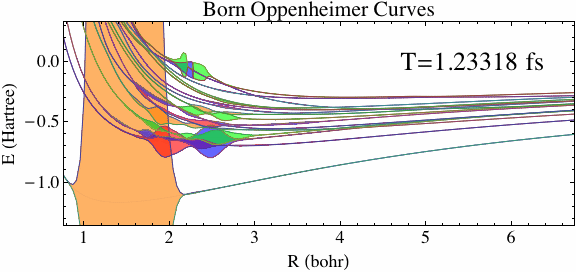
\includegraphics{MathLanCurves0_1_TimGayPi_10spf-1frame.png} \qquad\qquad\qquad}
\end{center}
%\end{figure}
}

%

\author{D. J. Haxton  \ \ C. W. McCurdy  \ \ T. N. Rescigno \ \ K. V. Lawler  \ \ J. Jones \ \ B. Abeln \ \  X. Li \\
{\small\em \copyright \  Draft date \today }
\date{ }}
\begin{document}




\maketitle

LBNL-AMO-MCTDHF is a suite of codes for Multiconfiguration Time-Dependent Hartree-Fock applied
to ultrafast laser dynamics of atoms and molecules.
%to atoms and molecules.
It calculates nonadiabatic electronic and nuclear wave functions
for the nonrelativistic Schr\"odinger equation.  Currently it uses the dipole approximation in length and velocity gauge and has options for a variety
of laser pulses.  It contains analysis and output routines and auxillary scripts 
for calculating absorption and stimulated emission, populations, total and partial photoionization, wave mixing,
and other capabilities.
It supports
%
\begin{itemize}[noitemsep]
\item{Electronic wave functions for atoms (\verb#chmctdhf_atom#)}
\item{Vibronic wave functions for diatoms using prolate coordinates (\verb#chmctdhf_diatom#)}
\item{Electronic wave functions for polyatomics with fixed nuclei (\verb#chmctdhf_sinc#)}
\end{itemize}
%
Future versions will support
\begin{itemize}[noitemsep]
\item{Electronic wave functions for atoms (\verb#chmctdhf_atom#)}
\item{Rovibronic wave functions for diatoms using prolate coordinates (\verb#chmctdhf_diatom#)}
\item{Rovibronic wave functions for diatoms using modified prolate coordinates (\verb#chmctdhf_diatom2#)}
\item{Vibronic wave functions for polyatomics and general Cartesian treatment (\verb#chmctdhf_sinc#)}
\end{itemize}
%
The method and equations are described in
%
\begin{itemize}[noitemsep]
\item{\textit{MCTDHF treatment of electronic and nuclear dynamics in diatomic molecules. }
D. J. Haxton, K. V. Lawler, C. W. McCurdy, Phys. Rev. A \textbf{83}, 063416 (2011)}
\item{\textit{Two methods for restricted configuration spaces within the MCTDHF method.}
D. J. Haxton and C. W. McCurdy, Phys. Rev. A \textbf{91}, 012509 (2015)}
\end{itemize}
%
Some of the largest nuts and bolts are due to
\begin{itemize}[noitemsep]
%
\item{\textit{{\sc Expokit.} {A} Software Package for Computing Matrix Exponentials.} R. B. Sidje, ACM Transactions on Mathematical Software 24, 130 (1998)}
\item{\textit{Adiabatic formulation of heteronuclear hydrogen molecular ion.} B. D. Esry and H. R. Sadeghpour, Phys. Rev. A 60, 3604 (1999)}
%\item{\textit{Numerical grid methods for quantum-mechanical scattering problems.}  T. N. Rescigno and C. W. McCurdy, Phys Rev A \textbf{62}, 032706 (2000)}
\item{\textit{Solving the three-body Coulomb breakup problem using exterior complex scaling.}  C. W. McCurdy, M. Baertschy, T. N. Rescigno, J. Phys. B. \textbf{37}, R137 (2004)}
\item{\textit{Grid-based methods for diatomic quantum scattering problems: A finite-element discrete-variable
representation in prolate spheroidal coordinates.}  L. Tao, C. W. McCurdy, T. N. Rescigno, Phys. Rev. A 79, 012719 (2009)}
\item{\textit{An efficient basis set representation for calculating electrons in molecules.}
J. R. Jones, F.-H. Rouet, K. V. Lawler, E. Vecharynski, 
 K. Ibrahim, S. Williams, B. Abeln, C. Yang,  D. J. Haxton, C. W. McCurdy, X. Li,  T. N. Rescigno, submitted.}        
        %
% Numerical grid methods for quantum-mechanical scattering problems 
%T. N. Rescigno1,2 and C. W. McCurdy2,3
%PHYSICAL REVIEW A, VOLUME 62, 032706 (2000)
%
\end{itemize}

%Applications and other:
%%
%\begin{itemize}
%\item{\textit{Population transfer between valence states via autoionizing states using two-color ultrafast $\pi$ pulses in XUV and the limitations of adiabatic passage.}
%X. Li, C. W. McCurdy, D. J. Haxton, Phys. Rev. A \textbf{89}, 031404(R) (2014)}
%\item{\textit{Ultrafast population transfer to excited valence levels of a molecule driven by x-ray pulses.}
%D. J. Haxton and C. W. McCurdy, Phys. Rev. A \textbf{90}, 053426 (2014)}
%\item{\textit{Single photoionization of Be and HF using the multiconfiguration time-dependent Hartree-Fock method.}
%D. J. Haxton, K. V. Lawler, C. W. McCurdy, Phys. Rev. A \textbf{86}, 0134106 (2012)}
%\end{itemize}

%\pagebreak

The original open-source MCTDH code of H.-D. Meyer \textit{et al.} at Heidelberg has driven our
interest in MCTDHF
%, inspired the structure of the code 
and guided this numerical implementation directly, providing
the foundation for the nomenclature and notation used here and in our articles in press, the input style, the variable names, and the layout of this manual.
Reviews and guides available at the MCTDH website may help fill in the blanks.
\begin{itemize}[noitemsep]
%
%\item{\textit{The multi-configurational time-dependent Hartree approach.} H.-D. Meyer, U. Manthe, L. S. Cederbaum. Chem. Phys. Lett. \textbf{165}, 73 (1990).}
\item{\textit{An efficient \& robust integration scheme for the equations of motion of the multiconfiguration time-dependent Hartree (MCTDH) method.}
M. H. Beck and H.-D. Meyer, Z. Phys. D \textbf{42}, 113 (1997)}
\item{\textit{The multiconfiguration time-dependent Hartree method: A highly efficient algorithm for propagating wavepackets.}
M. H. Beck, A. J{\"a}ckle, G. A. Worth, H.-D. Meyer, Physics Reports \textbf{324}, 1 (2000)}
\end{itemize}

LBNL-AMO-MCTDHF  has been funded 
primarily (2013-2018)
by the United States Department of Energy Early Career Program, 
WAS\#KC/CH57/5, and entirely
under U.S. D.O.E. contracts 
\#DE-FG02-94ER14413, % CHG
\#DE-AC02-05CH11231, % LBNL AND NERSC BOTH
and \#DE-SC-0007182. % UC Davis

This project is dedicated to the memory of Donovan Emil Smith.



%LBNL-AMO-MCTDHF Version 1.0 is dedicated to the memory of Donovan XXX Smith.


%U. Manthe, H.-D. Meyer, and L.S. Cederbaum.
%Wave-packet dynamics within the multiconfiguration Hartree framework: General aspects and application to NOCl.
%J.Chem.Phys. 97 (1992), 3199.




\tableofcontents




\chapter*{Preliminaries}


\section{Git install}

The code is distributed through GitHub.com.
Please visit 
\begin{quote}
    \verb#http://commons.lbl.gov/display/csd/LBNL-AMO-MCTDHF#
\end{quote}
to request access to the code.
Send us a message via this website.   We will receive the message and 
you will be added to Team Users on the LBNL-AMO-MCTDHF GitHub organization.  You will get an
email invitation when this happens.
%
Then you can view the repository on your browser
\begin{quote}
    \verb#https://github.com/LBNL-AMO-MCTDHF/V1#
\end{quote}
and perform a git clone to obtain the code.
\begin{quote} 
    \verb#prompt> git clone https://github.com/LBNL-AMO-MCTDHF/V1 master#
\end{quote}
%
Instead of git clone, you can download the zipfile
%
\begin{quote} 
    \verb#https://github.com/LBNL-AMO-MCTDHF/V1/archive/master.zip#
\end{quote}
The \verb#README# that is visible on the website and included with the code is included below, and includes quick installation
instructions for mac.


\begin{verbatim}

  ** LBNL-AMO-MCTDHF VERSION 1.27 **

v1.27 predictor/corrector algorithm modified; results will be different,
   depending on stepsize par_timestep

v1.27 work done by or on each pulse in Hartree output in various
   files for action 21 emission/absorption.  Circular polarization
   output added action 21 -- new &parinp namelist variable 
   act21circ.eq.0 default -- set act21circ.ne.0 to enable circular 
   polarization output

v1.26 angular differential partial photoionization, action 17, with
   angularflag.ne.0

v1.20 multiple cation files for partial photoionization action 17
   using numcatfiles, catspffiles, catavectorfiles in namelist &parinp
   cation.configlist.BIN no longer needed

v1.19 better improvedquadflag=2 and 3 (orbitals).  Excited states
   may be calculated more easily.

v1.18 predictor/corrector algorithm modified; results will be different,
   depending on stepsize par_timestep

v1.16 FACTOR OF 1/3 REMOVED FROM PHOTOIONIZATION (Actions 16,17)

   **** photoionization RESULTS WILL BE 3x GREATER NOW - BEWARE ****

   the factor of 1/3 is historical.  The cross section now reported
   in column 3 of xsec.spi.dat, xsec.proj.spi.datXXXX, is
   the quantum cross section in Megabarns for the problem at hand.
   Perform a 1:2 weighted average of parallel and perpendicular
   to obtain the cross section averaged over orientations

   The ionization and absorption cross section for H2 is about 12 Mb 
   at ion onset for both perpendicular and parallel.  Not 4.  He xsec
   is about 8.

ALSO v1.16 linear damping (fttriwindow=1) NEW DEFAULT actions 1,16,17,21
   RESULTS WILL BE DIFFERENT (hopefully better)
   Probably better results for absorption/emission, action 21.
   CONSIDER fttriwindow=0, ftwindowpower=2 in namelist &parinp
   to invoke old windowing function for actions 1,16,17.

ALSO v1.16 ABSOLUTE UNITS (megabarns) IMPLEMENTED FOR ACTION 21
   emission/absorption.  Column 9 in ZDipoleft.Dat etc is cross 
   section in Mb. See H2 and Helium examples.

ALSO v1.16 par_consplit.ne.0 attempted first time.  Total MPI 
   parallelization of LBNL-AMO-MCTDHF calculation with
   par_consplit.ne.0 and parorbsplit.eq.3 (parorbsplit.eq.3 for 
   polyatomic only)

CHANGES TO PULSE FOURIER TRANSFORM SUBROUTINES IN VERSION 1.10.
VARIABLES EFLUXLO, EFLUXHI, NEFLUX, FLUXNBINS, FLUXSINEOPT DEPRECATED.
NOTE NEW VARIABLE pulseft_estep USED FOR Pulseft.Dat OUTPUT ONLY

-----------------------------------------------------------------------
Please watch the commits to stay notified about bugs and bug fixes:
     https://github.com/LBNL-AMO-MCTDHF/V1/commits/master

Known bugs appear as issues:
     https://github.com/LBNL-AMO-MCTDHF/V1/issues
-----------------------------------------------------------------------

The scripts in the example directories use bash and gnuplot.  

Using the bash shell is recommended but may not be necessary.
To begin a bash shell, if it is not your default, simply execute the command
   prompt> bash
To set bash as your default shell on mac or other linux, execute the command
   prompt> chsh -s /bin/bash

Lots of scripts use gnuplot.  Gnuplot should be installed on your system,
if you want to have an easy time seeing the results of the example calculations.
If gnuplot is installed on your system then the command
   prompt> which gnuplot
should return the location of the executable file.  If it returns nothing then
it is not installed.  The best way to install gnuplot is probably with macports.

Possible workflow described below for mac.  The general idea is that you can 
   work entirely within the directory that you clone and to which you pull, not 
   copy the git distribution elsewhere for compilation.

----------------------------------------------------------------------------

On Mac: minimal demonstration.  *BIN*mac* directories use GFORTRAN.  You must have
gfortran installed to use the *BIN*mac* directories.  To install gfortran -- which
you will need to do if the Makeme step fails -- visit 

     https://gcc.gnu.org/wiki/GFortranBinariesMacOS

00)  mkdir V1
     cd V1
     git clone https://github.com/LBNL-AMO-MCTDHF/V1 master .

          or download using a web browser

     https://github.com/LBNL-AMO-MCTDHF/V1/archive/master.zip
          and unzip this file
     unzip master.zip
     mv master V1
     cd V1

     PERFORM ALL OTHER STEPS IN THIS V1 DIRECTORY.

0)   You must get the examples now separately.

     cd EXAMPLES-DEPOT
     rm README
     git clone https://github.com/LBNL-AMO-MCTDHF/examples-depot master .

          or download using a web browser

     https://github.com/LBNL-AMO-MCTDHF/EXAMPLES-DEPOT/archive/master.zip
          and unzip this file to get the EXAMPLES-DEPOT examples files.

1)   cd COMPDIRS/BIN.ecs.hermnorm.mac
     ./Makeme

     if this fails, you need gfortran.  Also you may then

     cd ../debug.BIN.ecs.hermnorm.mac
     ./Makeme
     cd ../BIN.ecs.hermnorm.mac.mpi
     ./Makeme
     cd ../debug.BIN.ecs.hermnorm.mac.mpi
     ./Makeme

     [ You can delete the directories in COMPDIRS that you don't want, e.g.
     cd COMPDIRS
     rm -r *BIN*law* *BIN*ediso* *BIN*cori* ]

2)   You need to have the code in your path.  Safe, temporary way:

2A)  cd COMPDIRS/BIN.ecs.hermorm.mac
     export PATH=$PATH:$PWD

2B)  Permanent way, system-wide, links in /opt/local/bin, requires root password:
     cd COMPDIRS/BIN.ecs.hermorm.mac
     ./LinkMe
     cd ../debug.BIN.ecs.hermorm.mac
     ./LinkMe debug
     cd ../BIN.ecs.hermorm.mac.mpi
     ./LinkMe mpi
     cd ../debug.BIN.ecs.hermorm.mac.mpi
     ./LinkMe mpi.debug

2C)  Permanent way, user-specific, script that edits your .bashrc file
     cd COMPDIRS/BIN.ecs.hermnorm.mac
     ./LinkMeLocal

     You must restart the terminal after step 2C.

3)   mkdir EXAMPLES
     cp -R -p EXAMPLES-DEPOT/H2-EXAMPLE-PLAIN-SCRIPTS EXAMPLES

4)   cd EXAMPLES/H2-EXAMPLE-PLAIN-SCRIPTS
     follow the README; 

     ./Relax.Bat
     ./Fourier.Bat 
     ./Flux.Bat 500
     ./gnu.xsec

     for total photoionization; see the README for more.
 
If you want to update the code then perform steps 5 and 6, like steps 1-4, 
in the V1 working directory,

5)   git pull https://github.com/LBNL-AMO-MCTDHF/V1
     git pull --tags https://github.com/LBNL-AMO-MCTDHF/V1

     then ./Makeme should be sufficient, in the BIN directories,
     but ./Makeme clean; ./Makeme would certainly be fail safe

6)   cd EXAMPLES-DEPOT
     git pull https://github.com/LBNL-AMO-MCTDHF/examples-depot
     git pull --tags https://github.com/LBNL-AMO-MCTDHF/examples-depot

If you want to switch versions of the code then do e.g.

     git checkout tags/v1.21
     cd COMPDIRS
     for dir in *BIN*; do cd $dir; ./Makeme clean; ./Makeme & cd ..; done

This should work for tags v1.16 and later.  Return to the most up-to-date 
version of the code by executing

     git checkout master

and again recompiling.

----------------------------    MODULES TO LOAD    -----------------------------
---------------------------- ON NERSC & LAWRENCIUM -----------------------------

  COMPDIRS/BIN.ecs.hermnorm.law,  COMPDIRS/BIN.ecs.hermnorm.edison, etc.

LAWRENCIUM:
  module load mkl

EDISON:
  module unload cray-libsci
  module load mkl
\end{verbatim}




%%
%%
%%\section{Quick Install}
%%
%%The code is provided with the following directory structure.  
%%%
%%{\footnotesize
%%\begin{verbatim}
%%prompt> tar -xvf MCTDHF.010115.VERSION1.0.tar.gz
%%prompt> cd MCTDHF.010115.VERSION1.0
%%prompt> ls
%%   LBNL-AMO-MCTDHF.pdf
%%   EXAMPLES
%%   JOB_SETUP_SCRIPTS
%%      TEMPLATES
%%   MCTDH.SRC
%%   COMPDIRS
%%      MCTDH.SRC -> ../MCTDH.SRC
%%      BIN.ecs.hermnorm.law.openmp.nofft
%%      debug.BIN.ecs.hermnorm.mac
%%      BIN.mac
%%      BIN.ecs.hermnorm.edison
%%\end{verbatim}}
%%%
%%etc.
%%
%%There are three directories at top level, \verb#MCTDH.SRC#, \verb#EXAMPLES#, and \verb#COMPDIRS#.  
%%The \verb#MCTDH.SRC# directory at top level contains the actual hard copy of the fortran code.  
%%The code is NOT compiled in \verb#MCTDH.SRC#.
%%There are many compilation directories ready-to-go for installation of the code on various machines, provided in \verb#COMPDIRS#.  
%%There are optimized versions, and versions with debugging flags.  Please compile the debugging version too and use it if the code
%%seems to be producing an invalid or unstable result, or actually crashes.  The supported machines, the machines with ready-to-go
%%directories in \verb#COMPDIRS#, are 
%%\begin{itemize}
%%\item{Lawrencium (extension \verb#.law#, e.g. \verb#BIN.ecs.hermnorm.law.openmp.nofft#).  Intel sandybridge, intel fortran compiler with mkl.}
%%\item{Edison on NERSC (extension \verb#.edison#, e.g. \verb#debug.BIN.ecs.hermnorm.edison#)}
%%\item{Mac (extension \verb#.mac#, e.g. \verb#debug.BIN.mac#)}
%%\end{itemize}
%%
%%You may delete the directories in \verb#COMPDIRS# that you don't want.
%%
%%All you need to do is go to the \verb#BIN# directory you want and run \verb#./Makeme#.  The code should then be compiled as, e.g.
%%{\footnotesize
%%\begin{verbatim}
%%prompt> mv COMPDIRS/*BIN*mac* .
%%prompt> rm -r COMPDIRS/*
%%prompt> mv *BIN*mac* COMPDIRS
%%prompt> cd COMPDIRS/BIN.ecs.hermnorm.mac
%%prompt> ./Makeme
%%prompt> ls
%%      .
%%      .
%%chmctdhf_sinc
%%chmctdhf_diatom
%%chmctdhf_atom
%%\end{verbatim}}
%%
%%Then you need to put the three programs in your \verb#$PATH# somehow so that you can use them in any working directory.  We recommend e.g.
%%{\footnotesize
%%\begin{verbatim}
%%prompt> echo $PATH
%%  /usr/bin:/usr/sbin:/opt/local/bin:/home/me/bin
%%prompt> cd ~/bin
%%prompt> ln -s ~/myprogs/LBNL-AMO-MCTDHF/V1.0.INTELFFT/COMPDIRS/BIN.ecs.hermnorm/chmctdhf_diatom ./chmctdhf_diatom
%%prompt> ln -s ~/myprogs/LBNL-AMO-MCTDHF/V1.0.INTELFFT/COMPDIRS/debug.BIN/mctdhf_sinc ./mctdhf_sinc.debug
%%\end{verb atim}}
%%etc.

\section{Running the code}

The code looks for an \verb#Input.Inp# input file.  If another input file is desired, use e.g. \\
\verb# > chmctdh_atom Inp=Input.Inp.myinput#

\

The code will perform a calculation with default parameters, if no input is given.

\section{File system etiquette\label{etsection}}

See also section \ref{act15sect} and note script \verb#findwork# at top level in the distribution.
\ \\ 
\ \\
If they do not exist in the working directory, the code makes the subdirectories 

\verb#WALKS#

\verb#Flux#

\verb#Dat#

\verb#Bin#

\verb#timing# \\
For more information on \verb#WALKS# see section \ref{outsection}, Output.  For more information on
\verb#Flux#, see  \ref{act15sect}.  \verb#Bin# is generally used to save the wave function, and generally \verb#Dat# contains
numerical text output from actions, section \ref{actsection}.  Timing output, what is discussed in section \ref{blah},
 is sent to directory \verb#timing# if \verb#&parinp# namelist variable \verb#notiming# is set less than the value 2,
 its default, and is described in section \ref{booga}.
 
 \
 
Some large files may end up in these directories.  Beware of this.  Again, 
see also section \ref{act15sect} and note script \verb#findwork# at top level in the distribution.
On a supercomputer e.g. NERSC machines, you \textbf{MUST} be reading and writing these files to the \verb#$SCRATCH# directory.  
One could run on the axl condo cluster home file system \verb#/clusterfs/axl# 
but make \textbf{symbolic links} to the scratch directory.  E.g.
\begin{verbatim}
> mkdir $SCRATCH/blah5
> ln -s $SCRATCH/blah5 ./WALKS
\end{verbatim}








\section{Run Control}
A running calculation can be stopped by creating a file named \verb#stop# in its working directory.  

%%
%%\section{Changes from version 0}
%%
%%\begin{itemize}
%%%
%%\item{There is a polyatomic version under development and compiled under \verb#chmctdhf_sinc#.  Namelist \verb#&sincparinp#.
%%\begin{itemize}
%%\item{This version is MPI parallelized over orbitals (totally).  Set both \verb#parorbsplit=3# in namelist \verb#&parinp# and \verb#orbparflag=.true.# in 
%%namelist \verb#&sinc_params# to do this.  
%%For the other versions of the code (\verb#chmctdhf_atom# and \verb#chmctdhf_diatom#) option \verb#parorbsplit=3# is not
%%supported and will result in an error.  If these options are set, \verb#numpoints# needs to be divisible by the number of processors.}
%%%
%%%\item{Always use \verb#toepflag=1# in
%%%\verb#&sinc_params#; this toes the Toeplitz trick with $T^{-1}$, not the kinetic energy.}
%%\item{Only cubic grids are supported.  There is only one variable, \verb#numpoints#, number of points on a side.}
%%\item{There are options for a complex absorbing potential, CAP, and approximate exterior complex scaling, 
%%ECS, in which the Coulomb operators are not scaled.}
%%\end{itemize}
%%}
%%%
%%\item{\verb#mcscfflag# is deprecated; there is no ``mcscf mode.''  There is still \verb#mcscfnum#, number of A-vectors relaxed or propagated.  
%%\textbf{You can propagate multiple A-vectors} and this may be important for some cases ... will discuss.
%%No \verb#mcscf.bin# is produced; everything is in \verb#spfs.bin# and \verb#avector.bin#.}
%%%
%%\item{There is the option \verb#littlesteps# to divide the A-vector propagation over the mean field timestep (\verb#par_timestep#).  This can be used
%%to optimize for speed.  It is needed if you want to
%%to try a big time step (\verb#par_timestep#) relative to the frequency of the pulse.  Big \verb#par_timestep#s are possible for weak pulses regardless of their
%%frequency using
%%\verb#littlesteps# $>$ 1. \textbf{Try bigger timesteps, with }\verb#littlesteps# $\mathbf{>}$\textbf{ 1, especially if your pulse is weak.} 
%%E.g. \verb#par_timestep=0.5d0# and \verb#littlesteps=10#.  Yes, for propagation!}
%%%
%%\item{ 
%%Try bigger time steps in general as lots of nuts and bolts have been tightened.  \verb#expotol# should be set low (stringent tolerance criterion), like 1d-8 or 1d-9, because
%%in the end it goes faster for the entire run with a stringent criterion anyway.
%%There is no need for \verb#exposteps# which has been deprecated.  But you may wish to optimize \verb#expodim# (starting Krylov dimension) and
%%especially \verb#maxexpodim# (its maximum value).
%%  If your orbital or a-vector iterations are restarting, as per \verb#expo.dat# or \verb#avecexpo.dat#, 
%%  you should be sure \verb#maxexpodim# or \verb#maxaorder# is high (but not too 
%%  high -- two or three hundred), but not worry if it is restarting after that.  See ``optimizing your runs'' below.}
%%%
%%\item{The variables \verb#nuccharge1#, \verb#nuccharge2#, \verb#lbig#, and \verb#mbig# are in namelist \verb#&heparinp# or \verb#&h2parinp#,
%%not \verb#&parinp#.}
%%%
%%\item{All polarizations in both gauges are now possible using \verb#pulsetheta# and \verb#pulsephi#.  \verb#pulsestrength# is complex-valued, which 
%%permits the use of nonphysical rotating waves.}
%%%
%%\item{\verb#whichprojflux# and \verb#corrflag# are deprecated.  The options for the Hanning window implemented by B. A. remain; 
%%whereas they were \verb#corrflag#=3 or 4 before, now the variable is \verb#hanningflag#=3 or 4, with other values having no effect.}
%%%
%%\item{\verb#improvedquadflag=1# is the option for doing Newton solve for the A-vector to converge excited states.  Options 2 and 3 are NOW REINSTATED (for orbitals).  2 = orbitals, 3 = both.}
%%\item{\verb#improvednatflag#=1 is fully debugged; it 
%%and \verb#improvedquadflag#=1 can be set at the same time reliably.  Note the message ``Vectors converged on read'' when performing
%%relaxation and \verb#sparseconfigflag#=1 that typically is printed each iteration as the relaxation is nearing convergence if one does
%%not alter the default \verb#lanthresh=1d-9#, even with \verb#improvednatflag#=1.}
%%%
%%\end{itemize}
%%%
%%Less important
%%\begin{itemize}
%%%
%%\item{\textbf{There is orbital parallelization.}  Running in parallel should speed the calculation regardless, unless you have a very small grid for the orbitals perhaps.
%%Variable \verb#parorbsplit#, default 1 (parallel).  Note the \verb#MPI# column in file \verb#timings/actreduced.time.dat#.  Not all aspects of the multiplication are
%%parallel; a good choice is \verb#nprocs#$=q\times$\verb#nspf#, with $q$ integer; then \verb#q# copies of the orbitals are propagated and MPI communication is among groups of
%%\verb#nspf# processors.}
%%%
%%\item{\verb#expodim# is now the starting dimension of the orbital propagation, and new variable \verb#maxexpodim# is its maximum value.  Likewise for \verb#aorder# and the new variable \verb#maxaorder#.}
%%%
%%\item{The nature of the stopping criterion \verb#stopthresh# for relaxation has been changed.  It now is independent of time step and a function of the rate of change of the orbitals.  It is more robust.  A typical value of 10$^{-5}$ should be good, 10$^{-4}$ for hard cases; as low as 10$^{-7}$ should work if you want to be sure things are converged.}
%%%
%%\item{Restricted configuration lists are good to go with \verb#constraintflag#=1 or 2, density matrix or Dirac-Frenkel.  BOTH require \verb#dfrestrictflag#=1 or greater.}
%%%
%%\item{There is a \verb#numskiporbs# variable in \verb#&parinp#, and \verb#num_skip_orbs# in \verb#&h2parinp# / \verb#&heparinp#.  They have different meanings: 
%%orbitals on file to skip, in the first case, and core orbitals to skip per m value for the generation of initial orbitals, in the latter cases.}
%%\end{itemize}
%%%
%%Even less important
%%%
%%\begin{itemize}
%%%
%%\item{There is the flag \verb#orbcompact# in \verb#&parinp# set by default to zero.  This is a new option; you can try it if you want.
%%When spfrestrictflag.ne.0, i.e., when there are symmetry restrictions on the orbitals, and \verb#mbig# is not zero, we believe you can now do things
%%the fully best way by setting \verb#orbcompact=1#.  Things probably won't change, and it is not extensively debugged.  But, you will probably notice that it takes
%%fewer steps occasionally, if you examine \verb#expo.dat#.  Usually, it will be the same number of steps, and if you are doing things correctly with tight
%%error tolerances, all the numbers, the results, will probably be exactly the same.  \textbf{Calculations in which the Hamiltonian does not conserve the symmetries 
%%imposed on the orbitals are now possible.}  We believe it is programmed it up correctly.  In other words, with \verb#orbcompact=1#, \verb#spfrestrictflag=1#,
%%\verb#spfugrestrict=1#, a calculation done with a heteronuclear diatomic, or a pulse, is being done correctly, we hope.  
%%With \verb#orbcompact=0#, it is not.
%%This is exotic; don't try it without discussing it; we want to do it to see if we can get the Fluorine atom to photoionize correctly.}
%%%
%%\item{\verb#timefac# is set internally according to \verb#improvedrelaxflag#.  Has no effect in \verb#&parinp# except if \verb#timefacforce# isn't zero.}
%%\item{The code can be compiled with script \verb#Makeme# in e.g. \verb#BIN.ecs.hermnorm#.}
%%\item{The code is now linked separately making a version for each coordinate system, and the F has been added to the name.  
%%E.g. \verb#chmctdhf_atom#, not \verb#chmctdh#.  \verb#atomflag# is deprecated.}
%%\item{The DVR for spherical polar coordinates has been changed.  Results will not be identical.}
%%%\item{The integrator has been rewritten.  It does not perform exactly the same which we did not figure out.  The default option is \verb#cmfmode#=0.  There
%%%are now two other variations on the mean field integrator that can be chosen with \verb#cmfmode#=1 and 2.  Try these if things are going wonky.  Mode 2 is mode zero plus an
%%%additional A-vector step.}
%%\end{itemize}
%%


\section{Optimizing your runs}

%Don't waste your time running bigger primitive basis calculations than are necessary.  Check the timing output to see where and why the calculation is running slow.  If necessary increase \verb#maxexpodim# or \verb#maxaorder# and perhaps \verb#expodim# or \verb#aorder#.  \textbf{Restarts of Krylov iterations are okay for propagation}; only bad for \verb#improvedquadflag# improved relaxation.  But they do make it slower, so increase the maximum dimensions to several hundred and you should get the best performance.

To successfully use the LBNL-AMO-MCTDHF package you must pay attention to timings.  The mean field treatment has
several components and it is necessary to intelligently select the basic parameters of the propagation, which are among
the \verb#&parinp# namelist variables, to achieve best performance.

\

A basic part of the mean field implementation is the separation of the orbital and A-vector propagation.  The orbitals
and the A-vector are propagated separately over a small time step, the mean field time step, the \verb#&parinp# namelist
variable \verb#par_timestep#.  Thus, a basic question is, which is taking longer, orbital propagation or A-vector?

\

We recommend performing rough draft calculations with grids as low-resolution as possible, such that the orbital calculation
runs fast.  We recommend not attempting to ``converge'' with respect to number of orbitals, namelist variable \verb#nspf#.
For first row diatomics, the ten-orbital calculation is the obvious starting point.  However, if more orbitals are desired, the
A-vector propagation may begin to take the majority of the computation time.

\

For the polyatomic version \verb#chmctdhf_sinc#, you will find best performance using one process per node (as opposed to
one process per core, for \verb#chmctdhf_atom# and \verb#chmctdhf_diatom#, which are generally run as sequential programs,
not parallel).  There are both vectorized (xSSE4.2, with intel FFT) and OpenMP (using FFTPACK) 
compilation directories provided for the lawrencium machine in \verb#COMPDIRS#.  The sequential (no shared memory, only
MPI parallelization) version is directory \verb#BIN.ecs.hermnorm.law.seq#.  On this machine \verb#$OMP_NUM_THREADS# controls
the number of threads per process and for the vectorized and OpenMP versions, all threads are taken if it is not set.

\

To ask the question, ``what is the breakdown in timings for my run?'' please set \verb#&parinp# namelist variable \verb#notiming=0#.
The code will answer, proceeding to output large amounts of information into separate text files in the
\verb#timing# directory.  See sections \ref{etsection} and \ref{act15sect} on file system etiquette.


\begin{itemize}
%
\item{There is \verb#Main.time.dat# but it should show that the time is all spent
in propagation.  Below you see there were about 6000 time units spent at the beginning, counted under Non MPI.
MPI +Non MPI is the total time and if the parallel propagation is working ok then MPI (communication) should be smaller
than Non MPI (computation).  If you don't include the startup time which is only counted in the MPI and Non MPI columns,
roughly speaking,
MPI+ Non MPI should add to the sum of the others.  TO-DO: ADD BIORTHOGONALIZATION COLUMN.
%
{\footnotesize
\begin{verbatim}
                       Spfs           Prop            Act          Final             MPI        Non MPI
        0.000             0            508              0              2             16           6381
        0.050             0            857              0              5             23           6726
                                                   .
                                                   .
        2.150             0          10362              0            121            232          16139
        2.200             0          10539              0            124            242          16310
\end{verbatim}}       
}
%
\item{To see the breakdown of the \verb#Prop# column, examine \verb#cmf_prop.time.dat#:
{\footnotesize
\begin{verbatim}
           Time      matel     denmat    reduced    spfprop      aprop    advance  constrain    #DERIVS
 T=       0.100         40          2          0        146        640          3          0         81
 T=       0.150         61          4          0        229        865          5          0         80
 T=       0.200         81          5          0        282       1090          7          0         48
 T=       0.250        103          6          0        360       1315          9          0         58
 T=       0.300        124          8          0        424       1539         10          0         58
 T=       0.350        145          9          0        521       1763         12          0        104
 T=       0.400        166         10          0        592       1988         14          0         63
 T=       0.450        186         12          0        664       2213         16          0         63
\end{verbatim}}
If A-vector propagation is taking quite a bit longer than orbital (spf) propagation, as above, run in parallel and try both \verb#parorbsplit#=0 and 1
if you want to be systematic and agnostic about it. \textbf{If matrix elements, density
matrices, or any of the in-between steps are taking a long time, CERTAINLY consider using a large} \verb#par_timestep#
\textbf{and} \verb#littlesteps#$\bm{>1}$.
 Most of the time is usually taken
in orbital propagation, in which case \verb#par_timestep# shouldn't affect overall speed that much, unless very small.  \begin{verbatim}#DERIVS\end{verbatim} is the number
of evaluations of the mean field operator required to take the time step (both predictor and corrector **CHECK**) and should never get too much bigger than 
$400 \times 2 = 800$ or so.  To get time per mean field evaluation, divide the other columns by the number of \verb#DERIVS#.}
%
\item{The timing file \verb#actreduced.time.dat# is very important and tells about column ``\verb#spfprop#'' in \verb#cmf.prop.time.dat# above.
However, note that this column \verb#spfprop# is not only \verb#actreduced#, which is the name of a subroutine; 
there is also the operation of the projector, which is counted
separately, and so to see the breakdown of column \verb#spfprop# in \verb#cmf.prop.time.dat#, go to \verb#jacoperate.time.dat#, note that
the first column is quite a bit smaller than the second of the two columns, and then look at \verb#actreduced.time.dat# which goes like this:
{\footnotesize
\begin{verbatim}
                  rmult       ke      pot     pulse     nuc     twoe  invdenma project  constrai     MPI 
T=       0.4500      169      881       88      106        0      318       18        4        0       55
T=       0.1500      333     1688      177      212        0      632       35        8        0      110
T=       0.3500      496     2496      266      318        0      947       52       12        0      165
T=       0.6500      659     3303      355      424        0     1261       69       16        0      219
\end{verbatim}}
Note that there are two steps to the mean field propagation of the orbitals, 
the predictor step and the corrector step, 
so the times, the first numerical column, may not be in order.  Orbital parallelization with \verb#parorbsplit# set nonzero should affect the columns
\verb#ke# through \verb#twoe# because those refer to steps that are distributed over processors by this option.  Generally speaking, with \verb#nprocs#=\verb#nspf#,
if the orbital parallelization is working well you should observe that the steps \verb#rmult#, perhaps \verb#invdenmat#, and \verb#MPI# take a significant proportion of the time.
}
\item{Examine \verb#expo.dat# which tells you about the orbital propagation.  
In the example below, notice the numbers 1 and 48 at the bottom.  That's one Krylov iteration, no restarts, with 48 matrix-vector multiplications required.
This is the output near the start of the run.  It has increased the krylov dimension up to 46 and at that point it does not need to restart, whereas
at the first step it required 2 steps, one restart, with 66 matrix vector multiplications total.  There have been steps rejected.  This
will happen at the beginning of the run when it is adjusting the internal step size, but should NOT happen afterwards that much.  If it is, something is wrong.  It will increase
the Krylov order (\verb#thisexpodim# as reported below) from where it starts (namelist input \verb#expodim#) up to
the maximum krylov order (namelist input \verb#maxexpodim#), and then if it is restarting then the number of steps will be greater than one, 
but it should not be rejecting steps and changing its stepsize.  In a nutshell: increase \verb#maxexpodim# up to 300, or something like that, and then if it is restarting, 
(steps $>$ 1) so be it, but it should not be rejecting steps very often, after the start of the run.  Consider increasing \verb#littlesteps# if you are trying to take big steps (large \verb#par_timestep#).
%
{\footnotesize
\begin{verbatim}
 Go Orbital Expoprop.  Tinit=  0.100000000000000       thisexpodim=          31 
  step   5.000000000000000E-002
       ...REJECTED  0.5000E-01  0.3849E-06  0.1000E-05
       ...REJECTED  0.4000E-01  0.1023E-06  0.1000E-05
    End expo. Orthog error, steps, stepsize, iterations  6.050711511541938E-015
           2  3.200000000000001E-002          66
 
 Go Orbital Expoprop.  Tinit=  0.100000000000000       thisexpodim=          38 
  step   5.000000000000000E-002
       ...REJECTED  0.5000E-01  0.2653E-06  0.1000E-05
    End expo. Orthog error, steps, stepsize, iterations  6.213364751595364E-015
           2  4.000000000000001E-002          80
 
 Go Orbital Expoprop.  Tinit=  0.150000000000000       thisexpodim=          46 
  step   5.000000000000000E-002
    End expo. Orthog error, steps, stepsize, iterations  1.136962511459106E-014
           1  4.999999999999999E-002          48
\end{verbatim}}
}
\item{Check file \verb#avecexpo.dat#, for the A-vector propagation, similar to \verb#expo.dat# above.}
%
\item{If running in parallel, check to be sure you get the same results (certainly to six digits for everything) for different numbers of processors.}
\item{ \verb#improvednatflag# to enforce natural orbitals for relaxation has been extensively debugged but it involves a difficult transformation of
the wave function.  For very large A-vectors, especially, be sure it is working ok; do the run without the flag as well. 
It is conceivable that the biorthogonalization routine could require tweaking for difficult cases, using the variables \verb#biodim# and \verb#biotol#.
The only two reasons, in general, for which  one \textit{needs} to use this option \verb#improvednatflag# in general is if, first,
one is going to perform excitations or annihilations subsequently -- or alternatively, second, if using density
matrix constraint (\verb#constraintflag=1#) in the subsequent propagation step.}
\item{\textbf{Try larger time steps} as described above. If you have a high frequency or strong laser and you are trying to take large time steps (e.g. for big A-vector), 
try the new variable \verb#littlesteps# $>$ 1 which may improve accuracy and stability in addition to speed, as described above.}
\item{Use the smallest primitive basis possible until you are doing production runs.  Go as small as you can without much static appearing in your result.  First 
make sure things are qualitatively right. \textbf{Absolute energies are not relevant.  Gauge dependence is.} Don't sweat getting transitions energies right, unless something is qualitatively
wrong.  Often transition/ionization energies can be off by an eV or more.}
%
%\item{\textbf{For excited state convergence (}\verb#improvedquadflag#\textbf{=1, 2, or 3) we recommend performing a run with} \verb#spf_flag#=0 \textbf{and using it as a guess for one %with} \verb#spf_flag#=1.  Remember to use a sufficient \verb#aorder#.  It will give a clear warning if the Krylov iterations are restarting, which in this case is bad.}
\end{itemize}


\section{Nomenclature}

Here are some quick statements about the terms used in this manual.

\

We sometime use the terms configuration and Slater determinant 
interchangeably.  Sometimes when we write configuration, we mean either a Slater determinant or a spin adapted sum
of Slater determinants.  But usually, we just mean Slater determinant.

\

The wave function is made of a time dependent linear combination of Slater determinants.  The coefficients in the linear
combination are time dependent.  The Slater determinants are also time dependent, because they are made of orbitals
that are time dependent.  Sometimes (with \verb#allspinproject=1#, default) the spin symmetry of the wave function is
enforced.  Then, the wave function is first represented as a linear combination of spin adapted linear combinations (SALCs
is an acronym we have seen) of Slater determinants.  Those linear combinations, the SALCs, are computed when the code starts.

\

So, not worrying about whether or not we are discussing Slater determinants (\verb#allspinproject=0#) or spin adapted linear
combinations thereof (\verb#allspinproject=1#), we will generally use the term ``configuration.''  

\

Again, we borrow from the MCTDH implementation of the Heidelberg group for not only the notation used in the equations,
but also the terms by which they are referred to and often even the variable names in the code.

\
 
Orbitals are the same thing as single particle functions, SPFs.  The configuration coefficients
are the ``A-vector,'' $\vec{A}$.  We have one- and two-electron reduced density matrix operators $\rho$ and $\Gamma$,
the reduced potential $\mathbf{w}$,
the reduced mean field operator
$\mathbf{W}_{\alpha\beta}=\sum_{\gamma\delta} \Gamma_{\alpha\beta}^{\gamma\delta}\mathbf{w}_{\gamma\delta}$, and
the one-electron Hamiltonian $h_0$.  The orbitals are $\vec{\phi}$; the coefficients of $\phi_\alpha$ are $\vec{c}_\alpha$.

\

For restricted configuration spaces, in which the orbitals are constrained to rotate into one another, we compute the 
$g_{\alpha\beta}=\langle \phi_\alpha \vert i\frac{\partial}{\partial t} \vert \phi_\beta \rangle $ matrix.  The matrix elements of $g$
among configurations are called $\tau$.

\begin{equation} \nonumber
i\frac{\partial}{\partial t} \vec{A} = (H - \tau) \vec{A}
\end{equation}
\begin{equation} \nonumber
%
%i\frac{\partial}{\partial t} \vec{\phi} = \left [ (1-P) \rho^{-1} \mathbf{W} + g \right] \vec{\phi}
%
i\frac{\partial}{\partial t} \vec{\phi} = \left [ (1-P) \left( \rho^{-1} \mathbf{W} + h_0 \right) + g \right] \vec{\phi}
%
\end{equation}


\chapter{Installation\label{installchapter}}

System administrators may use this section for very quick startup especially on supported machines.  Users may proceed to the next section.

\

The directory structure of the code makes extensive use of symbolic links and if you copy the directories you should ensure that you maintain 
the symbolic link structure.  On mac, use \verb#cp -R# to copy links as is.  Otherwise, they are copied as new files, and you have duplicates.  
This is not a big deal, but it can be a waste of space and if you update the file then you have inconsistencies.  You want to keep one copy of the files only.
Look at the directories, see the symbolic links, and then proceed to use these instructions:

\

The code is provided with the following directory structure.  The result of the \verb#ls# command is schematic and embellished to give you the idea.
%
{\footnotesize
\begin{verbatim}
prompt> tar -xvf MCTDHF.010115.VERSION1.0.tar.gz
prompt> cd MCTDHF.010115.VERSION1.0
prompt> ls
   LBNL-AMO-MCTDHF.pdf
   EXAMPLES
      H2PHOTO
   JOB_SETUP_SCRIPTS
      corotating_counterrotating_streaking.py
      TEMPLATES
         mpilaunchjob.slurm.template
         atomfile.txt
         Relax.Bat.template
   MCTDH.SRC
      DFFTPACK
         zfftf1.f
      SINCDVR
         sincDVR.f90
      H2PROJECT
         H2_params.f90
   COMPDIRS
      MCTDH.SRC -> ../MCTDH.SRC
      BIN.ecs.hermnorm.law.openmp.nofft
         Definitions.INC
         Name.Txt
         Makefile.header -> ../MCTDH.SRC/Makefile.header.lawrencium.openmp.nointelfft
         Definitions.ALL -> ../MCTDH.SRC/Definitions.ALL
         mctdhf.F90 -> ../MCTDH.SRC/mctdhf.f90
         DFFTPACK
            Makefile.header -> ../Makefile.header
            Makefile -> ../../MCTDH.SRC/DFFTPACK/Makefile
            zfftf1.f -> ../../MCTDH.SRC/DFFTPACK/zfftf1.f
         SINCDVR
            Makefile.header -> ../Makefile.header
            Makefile -> ../../MCTDH.SRC/SINCDVR/Makefile
            sincDVR.f90 -> ../../MCTDH.SRC/SINCDVR/sincDVR.f90
      debug.BIN.ecs.hermnorm.mac
      BIN.mac
      BIN.ecs.hermnorm.edison
\end{verbatim}}
%
etc.

There are three directories at top level, \verb#MCTDH.SRC#, \verb#EXAMPLES#, and \verb#COMPDIRS#.  
The \verb#MCTDH.SRC# directory at top level contains the actual hard copy of the fortran code.
There are many directories ready-to-go for installation of the code on various machines, provided in \verb#COMPDIRS#.  
There are optimized versions, and versions with debugging flags.  Please compile the debugging version too and use it if the code
seems to be producing an invalid or unstable result, or actually crashes.  The supported machines, the machines with ready-to-go
directories in \verb#COMPDIRS#, are 
\begin{itemize}
\item{Lawrencium (extension \verb#.law#, e.g. \verb#BIN.ecs.hermnorm.law.openmp.nofft#).  Intel sandybridge, intel fortran compiler with mkl.}
\item{Edison on NERSC (extension \verb#.edison#, e.g. \verb#debug.BIN.ecs.hermnorm.edison#)}
\item{Mac (extension \verb#.mac#, e.g. \verb#debug.BIN.mac#)}
\end{itemize}

You may delete the directories in \verb#COMPDIRS# that you don't want, but they don't take any space.

All you need to do is go to the \verb#BIN# directory you want and run \verb#./Makeme#.  The code should then be compiled as, e.g.
{\footnotesize
\begin{verbatim}
prompt> mv COMPDIRS/*BIN*mac* .
prompt> rm -r COMPDIRS/*
prompt> mv *BIN*mac* COMPDIRS
prompt> cd COMPDIRS/BIN.ecs.hermnorm.mac
prompt> ./Makeme
prompt> ls
      .
      .
chmctdhf_sinc
chmctdhf_diatom
chmctdhh_atom
\end{verbatim}}

Then you need to put the program in your \verb#$PATH# somehow so that you can use it in any working directory.  We recommend
{\footnotesize
\begin{verbatim}
prompt> echo $PATH
  /usr/bin:/usr/sbin:/opt/local/bin:/home/me/bin
prompt> cd ~/bin
prompt> ln -s ~/myprogs/LBNL-AMO-MCTDHF/V1.0.INTELFFT/COMPDIRS/BIN.ecs.hermnorm/chmctdhf_diatom ./chmctdhf_diatom
prompt> ln -s ~/myprogs/LBNL-AMO-MCTDHF/V1.0.INTELFFT/COMPDIRS/debug.BIN/mctdhf_sinc ./mctdhf_sinc.debug
\end{verbatim}}

There are four versions of the code with different datatypes, but \verb#chmctdhf# is all that is generally needed.  Compilation directories 
are provided for \verb#chmctdhf# and \verb#mctdhf# only.
\begin{itemize}
\item{\verb#mctdhf# : REAL VALUED VERSION FOR RELAXATION. (e.g. \verb#BIN.mac#) }
\item{ \verb#pmctdhf# : COMPLEX VALUED, PROPAGATION WITHOUT ECS (e.g. \verb#BIN.complex.mac#)}
\item{ \verb#chmctdhf# : COMPLEX VALUED, WITH ECS: USUAL VERSION (e.g. \verb#BIN.ecs.hermnorm.mac#)}  
\item{ \verb#cmctdhf# : COMPLEX VALUED, ECS, C-NORM: FOR RESONANCE RELAXATION (e.g. \verb#BIN.ecs.cnorm.mac#)}
\end{itemize}

If you are using an architecture different from all of these machines, then you should make a new \verb#BIN# directory and a new \verb#Makefile.header.mymachine#
in \verb#MCTDH.SRC#, linking the new header file as \verb#Makefile.header# in the new \verb#BIN# directory.
There are parallel versions of \verb#Makefile.header# for mac already done.
Your fortran compiler must support the C preprocessor.  You may have to figure out flags to invoke it.
If you want to run the calculation in parallel (there is now some orbital parallelization!)
then in Makefile.header 
you must include the line "\verb#MPIFLAG = -D MPIFLAG#"  and include
paths or flags in 
variables \verb#MYINCLUDE# and \verb#LAPACK# if needed.  Intel FFT libraries may be used by setting \verb#FFTFLAG = -D INTELFFT#.
Portland group compilers require \verb#PGFFLAG = -D PGFFLAG#.



\chapter{Input}

 The code is run from the command line and takes command line arguments and also parameters from an input file, by default \verb#Input.Inp#.  
 Command line arguments supersede input from file.
 All variables that can be set are listed in Sec.~\ref{varsect}.
 %
To use an input filename different from \verb#Input.Inp#, specify it as follows:
\begin{quote}
{\small\begin{verbatim}
C:> chmctdhf_atom Inp=Input.Inp.myinput
\end{verbatim}}
\end{quote}
%
If \verb#Input.Inp# or the specified input filename does not exist it will do a default calculation.  One can specify multiple command 
line arguments, e.g.
\begin{quote}
{\small 
\begin{verbatim}
C: > chmctdhf_atom Inp=Input.Inp.awesome T=1000.0 Nspf=4 Act=1
\end{verbatim}}
\end{quote}



\section{Namelist input}

Fortran includes a feature that makes it easy to input variable values from file, called namelist input.  It is not case sensitive.  
Variable names in the namelists in the input file are the same as their names in the code.  There are four 
namelists that can be used as input in the input file (default \verb#Input.Inp#).   The complete list of variables that can be set are listed in Sec.~\ref{varsect},
which is a printout of \verb#parameters.f90# with comments.  You can also look at the code: for instance,
the \verb#&parinp# namelist variables can be seen in \verb#getparams.f90#, subroutine getparams(); that's where the \verb#&parinp# namelist is defined.

\

{\large \textbf{** In your input file: **}}
\begin{itemize}
\item{You must have namelist \verb#&parinp#.}
\item{If variable \verb#tdflag# in namelist \verb#&parinp# is set to 1 (including a time-dependent pulse), or if doing a flux analysis calculation
(action 16 or 17) (except if \verb#noftflag# is set nonzero in \verb#parinp#), you must also have namelist \verb#&pulse#.}
\item{You must have \verb#&h2parinp# for diatoms (\verb#chmctdhf_diatom#), \verb#&heparinp# for atoms (\verb#chmctdhf_atom#), or 
\verb#&sincparinp# for polyatomics (\verb#chmctdhf_sinc#).}
\end{itemize}





\section{Specifying the wave function}

The orbitals and A-vector are specified independently.  One may load either of them, or obtain them by diagonalization.
For orbitals, the core Hamiltonian is used for diagonalization.  One needs to specify the symmetry constraints for each.
Restricting the symmetry of the A-vector requires restricting the symmetry of the orbitals, but not vice-versa.

\subsection{Symmetry constraints}


By default the $S_z$ spin angular momentum projection quantum number is restricted.  It is specified by \verb#restrictms=X#.  This is $2\times$ the $S_z$ quantum number.  

By default the wave function is restricted to be an eigenfunction of spin, $\hat{S}^2$, via \verb#spinwalkflag=1# and \verb#allspinproject=1#.  
The high spin case is calculated ($S=M_s$).  Thus one specifies the multiplicity by setting \verb#restrictms# = multiplicity-1, i.e. for a doublet, \verb#restrictms#=1.

One generally wants to restrict spatial symmetry as well.  
To restrict the $l_z$ quantum number (angular momentum projection) of the orbitals set \verb#spfrestrictflag=1#.  
Then specify the $m_z$ values of the orbitals by \verb#spfmvals=0,1,-1,..#.
To restrict the parity of the orbitals set \verb#spfugrestrict=1#.  Then specify the parity by \verb#spfugvals=1,-1,0,0,...#
where 0 means no parity restriction.  

Without \verb#spfrestrictflag=1#, \verb#spfmvals# is only used if you are starting
from core orbitals, for your initial relaxation run for instance, in which case it is just used to select the initial orbitals.
Similarly for \verb#spfugrestrict#.

To restrict the overall angular momentum projection $L_z$ of the wave function, \verb#spfugrestrict# must be set nonzero;
then set \verb#mrestrictflag#=1 and \verb#mrestrictval# to $L_z$.  Similarly with \verb#ugrestrictflag# and \verb#ugrestrictval#.

To restrict $L_z$ to a \textit{range} of values, do not set \verb#mrestrictflag#; instead set \verb#mrestrictmin# and \verb#mrestrictmax#.  This is useful for relaxation
or propagation of multiple wave functions. \textit{See warnings in the section on relaxation.}

If one is reading in orbitals from file and \verb#spfrestrictflag# or \verb#spfugrestrict# is set, then the angular momentum projections or parities of the
orbitals must match those in the present calculation.

\subsection{Restricted configuration spaces}

Restricted configuration spaces, non-full-configuration interaction,
are a new capability and the numerical implementation is more difficult than the full CI method.  There are more things to do, and the integrator
ends up taking more steps to calculate the more rapidly changing orbitals.  There are profound issues relating to symmetry broken solutions of 
a relaxation calculation, to prepare the initial state, and therefore we advise using the real-valued versions \verb#BIN/mctdhf_XXX# to prepare the
initial state, or at least checking that the same energy is obtained with both complex and real versions.

For these reasons using restricted configuration spaces
be avoided until you have pushed the limit of a one node calculation.  Doing the code in parallel over many nodes is not something we want
to do if we want to make the best use of computer time.
For instance, with neon, with greater than 14 orbitals, one is going to need
a restricted configuration space, despite the use of \verb#sparseconfigflag=0#, \verb#sparseopt=0#, and small values for Krylov space parameters
(\verb#maxaorder#, \verb#aorder#, even \verb#maxexpodim# if the orbitals take up some space that can be freed).

You can also try frozen orbitals, \verb#numfrozen#, which reduces the number of electrons in your full CI calculation,
to avoid having to use a restricted configuration space.
 Frozen orbitals work, but they also require more things to do, slowing the calculation down,
and make the problem more numerically difficult.  \textit{But, if you want, do try frozen orbitals if your physics does not perturb the core orbitals! } 
This will require consultation as the manual is not complete.  See section~\ref{frosect}.

\

There are two methods for restricted configuration spaces (see the paper).  Density matrix (\verb#constraintflag=1#) and dirac-frenkel (\verb#constraintflag=2#).
A restricted configuration space can be used with \verb#constraintflag=0#, such that the $g$/$\tau$ matrix remains set to zero, 
but one is making uncontrolled error in the wave function.

\

With \verb#constraintflag# not equal to zero, \verb#dfrestrictflag# must be set nonzero.  Unless you are running action 22, it should be set \verb#dfrestrictflag=1#.

\

Then, \textbf{ALL THE FOLLOWING VARIABLES} 
should be incremented by the chosen value of \verb#dfrestrictflag#.  That is because, in the code, they
will be decremented by that amount, to obtain the included list of configurations.
 ``Incremented by 1'' means, change the value by 1 in the direction that enlarges the restricted configuration
space.  

\begin{verbatim}
minocc
maxocc
numexcite
vexcite
\end{verbatim}

\

Variables (namelist \verb#&parinp#) specifying a restricted configuration list are as follows.
The variables \\
\begin{tabular}{l}
\qquad \verb#numshells#\\
\qquad \verb#shelltop# \\
\end{tabular} \\
come first.  They divide the \verb#nspf# orbitals into shells.  By default there is one shell, \verb#numshells#$=1$, 
and \verb#shelltop(1)#$=$\verb#nspf#.
 \verb#shelltop# denotes the last spatial orbital in each shell.  You must enter \verb#shelltop# for shells 1 through numshells-1.  The value of shelltop for the last shell is automatically set to \verb#nspf#.  
 
 \
 
One way of doing a restricted configuration list, is to use one or the other or both of the two variables
\begin{tabular}{l}
\qquad \verb#numexcite# \\
\qquad \verb#vexcite#  \\
\end{tabular} \\
and leave it at that. 
Variable \verb#numexcite# may be set for shells 1 through numshells-1; \verb#numexcite#(i) corresponds to the maximum number of holes in shells 
1 through $i$ (so the list, if \verb#numshells#$>2$, should be never decreasing).  
\verb#vexcite# is the opposite of \verb#numexcite# and is only input for the last shell; it
corresponds to the maximum number of electrons in the last shell and so can be used 
to easily restrict the configuration list to all singles and doubles (CISD), etc.  

\

The other available options are \verb#minocc# and \verb#maxocc# which can be input for shells 1 through \verb#numshells#.
These are minimum and maximum occupation numbers.

\

To reiterate, \verb#vexcite#, \verb#numexcite#, \verb#minocc#, and \verb#maxocc# must all be incremented by the value of \verb#dfrestrictflag#
(1, unless using action 22, or unless debugging) from what you want them to be for the restricted configuration space you want. The configuration
lists are built using the incremented values, but the wave function is constrained to occupy only the restricted configuration space you want.
 If you are just
playing around and \verb#constraintflag# and \verb#dfrestrictflag# are both zero then just set these variables how you want them; you can do that,
but you are making uncontrolled error.

\

\textbf{TO PREPARE THE INITIAL STATE:}  To prepare the initial state for a propagation with the
density matrix constraint (\verb#constraintflag=1#), 
perform a relaxation calculation with \verb#improvednatflag=1#, \verb#constraintflag=0#, \verb#dfrestrictflag=0#.
You could also set \verb#dfrestrictflag# to the same value (probably 1) that you use for the propagation, in which case
your values for \verb#vexcite#, \verb#minocc#, etc. will be the same.  But \verb#constraintflag=0#, \verb#improvednatflag=1#
 for density matrix
initial state calculation.
  For Dirac-Frenkel (\verb#constraintflag=2#),
perform a relaxation calculation with the restricted configuration space machinery just as done for propagation.  You may even 
find you have to do regular imaginary time relaxation calculation (\verb#improvedrelaxflag=0#, \verb#threshflag=1#).  For relaxation
or improved relaxation you will need small time steps.  Set \verb#constraintflag=2#, \verb#dfrestrictflag=1# (or whatever nonzero),
just like the propagation calculation.

\

Always, if you are indeed taking the bold leap into restricted configuration space calculations, you should definitely do it BOTH WAYS,
density matrix and dirac-frenkel, \verb#constraintflag=#1 and 2.
Hopefully they will both work and if they do, it is a powerful convergence check.  Remember that 
you can check the overlap between two time-dependent wave functions
using Actions 15 and 23.



\subsection{Specifying the initial orbitals}



By default the orbitals are obtained by diagonalizing the core hamiltonian.  These would be used for a relaxation calculation.  Thus, for a relaxation calculation, no extra input is required.

One loads orbitals from file with \verb#loadsppflag=1#.   
\begin{quote}
{\footnotesize 
\verb#&parinp# \\
\verb#  loadspfflag=1#\\
\verb#  spffile="Bin/spfs.bin.mine"#}
\end{quote}

By default, the orbitals are loaded from \verb#./Bin/spfs.bin#, the same file that is written at the end of a run.  In practice you would save this file elsewhere and specify its location as above.

If you are loading orbitals with \verb#loadsppflag=1# and there are fewer orbitals in \verb#spfs.bin# than in the calculation, then the additional orbitals are taken from core orbital eigenfunctions.  This is useful if you want to converge an excited state with a small number of orbitals first, then add orbitals to get a better wave function.

For a relaxation run, obtaining the initial guesses for the orbitals from core diagonalization, even if specifying \verb#spfmvals# and \verb#spfugvals# as appropriate, one may find that the initial guess orbitals are incorrect for the desired calculation.  For instance, the ordering of 3$s$ and 3$d_{z^2}$ will depend on small numerical errors.  One may skip over the orbitals as follows: say that you want the 1st, 2nd, and 5th orbitals for $m$=0 and the 1st and 3rd for $m$=$\pm$1.  One would specify
\begin{quote}
{\footnotesize 
\verb#&h2parinp# \\
\verb#  num_skip_orbs=3# \\
\verb#  orb_skip=3,4,2#\\
\verb#  orb_skip_mvalue=0,0,1#}
\end{quote}
Thus you list the orbitals to skip and the corresponding $m$-values.

To read in two or more small sets of orbitals to combine into one set (useful for
interacting fragment type description) use \verb#numspffiles# and \verb#spffile(1)#, etc.  For instance you might have a run with three orbitals and one with
four and you could combine these for a seven orbital calculation.  You can skip over orbitals that are read in this step, by specifying \verb#numskiporbs#,
in namelist \verb#&parinp#.

\subsection{Frozen orbitals \label{frosect}}

If your calculation is getting out of hand (can't fit on one node, in memory), 
and it only involves valence electron dynamics, then you have two options -- restricted configuration spaces, or frozen orbitals.
If it involves core electron dynamics, you only have the restricted configuration space option.
Otherwise, if you are really at this point, perhaps, try both.

Frozen orbitals work like this.  Variable \verb#numfrozen# in namelist \verb#&parinp# is number of frozen orbitals (spatial orbitals, containing
two electrons).  So you might start with a small full CI calculation.  Say Neon, 6 orbitals.  Don't do hartree-fock!  We do not have an actual fock Hamiltonian.
We are missing the ``scalar terms'' in the reduced operator $\mathbf{\hat{W}}$.  They do not matter when $(1-P)$ is put in front of them.  
Therefore we do not have a good 1s energy eigenfunction.  All we have is natural orbitals 
-- or, now, the Dirac-Frenkel constraint -- to define orbitals.

By ``define orbitals'' we mean, in better terms, ``resolve orbitals''.  Given the space of orbitals -- six, say, for neon, with an extra $3s$ orbital beyond
the Hartree-Fock -- resolve orbitals means specify a specific set of six orthonormal orbitals.

So, the easiest thing is to start with non-Hartree-Fock, \verb#improvednatflag=1# calculation, with the restricted configuration space (no need for
\verb#dfrestrictflag# nonzero).

Take the orbitals on disk, and read them in for a calculation with frozen orbitals.  Start with neon, six orbitals, then read those orbitals in,
with \verb#nspf=5#, \verb#numfrozen=1#.  \verb#nspf# is the number
of unfrozen orbitals.
That will do a calculation with one frozen orbital, and five unfrozen orbitals, starting with the six
orbitals from your first calculation; the frozen orbital is now the $1s$ natural orbital from the first calculation.  You can go on and add more orbitals.

Specify \verb#spfmvals# and \verb#spfugvals# only for the unfrozen orbitals.

So, you could have done \verb#nspf=8#, \verb#numfrozen=1#, and it would have loaded the six orbitals, then added three more (the p orbitals) 
gotten from diagonalization
of the core Hamiltonian.  
  
Going from six orbitals to \verb#nspf=13#, \verb#numfrozen=1#, one would
set the thirteen values of \verb#spfmvals# and \verb#spfugvals# appropriately, then, we think this is how it goes,
one would need to specify \verb#num_skip_orbs=1# and \verb#orb_skip_mvalue=0# in \verb#&h2parinp#
or \verb#&heparinp#, to get the usual set of fourteen orbitals. 

\subsection{Specifying the initial A-vector}

Similar to the orbitals, one may specify
\begin{quote}
{\footnotesize 
\verb#&parinp# \\
\verb#  loadavectorflag=1#\\
\verb#  avectorfile="Bin/avector.bin.mine"#}
\end{quote}

With \verb#mcscfnum# $>$ 1 the code propagates multiple A-vectors, but still uses only one set of orbitals.  
To read in multiple A-vectors for such a 
run, use \verb#numavectorfiles# and \verb#avectorfile(1)=#, etc.  

One may also excite or annihilate orbitals and the following subsections describe that.  

When the excitation or annihilation is performed, it is done so in terms of the spin orbitals and the spin value is not conserved.  What is obtained from the excitation or annihilation is then projected upon the spin value specified in \verb#restrictval#, if \verb#spinwalkflag#=1.

One should take care that the orbitals one is annihilating or exciting are meaningful.  If one does a regular improved relaxation run, the orbitals will
be arbitrarily mixed.  If you want to have meaningful molecular orbitals, use \verb#improvednatflag=1#
in namelist \verb#parinp# in the relaxation run; the orbitals will then be natural orbitals.  Fock eigenfunctions are not implemented. 




\subsection{Annihilation}

One may read in an $(N+1)$-electron wave function and then annihilate an electron.  

Use \verb#avectorhole=# in namelist \verb#&parinp#.
\begin{quote}
{\footnotesize 
\verb#&avectorhole=1# }
\end{quote}
This will annihilate the first spin orbital.  As it hapens the even numbered spin orbitals are spin up and the odd numbered are spin down.  So if one is
reading in a triplet wave function (\verb#restrictms=2#) into a doublet calculation (\verb#restrictms=2#) and annihilating an electron, because the
high spin case is calculated one annihilates a spin up electron, odd numbered, as above.

One may use a linear combination of hole wave functions.  This would be useful for annihilating the left or right core hole.  To do this specify
\begin{quote}
{\footnotesize 
\verb#&numholecombo=2# \\
\verb#&avectorhole=1,3# }
\end{quote}
This makes the (+) combination of orbitals (which each come out with an arbitrary phase).  To make the (-) combination use \verb#&avectorhole=1,-3#.

\subsection{Excitation}

One may read in an A-vector and then perform an excitation or annihilation.  

To perform an excitation, use \verb#avectorexcitefrom# and
\verb#avectorexciteto# in namelist \verb#&parinp#.  
These variables should be assigned to the spin orbital indices.  With the default value of \verb#orderflag#, this means
that to perform an excitation from the first spatial orbital, spin down, to the third spatial orbital, spin up,  you'd do \verb#avectorexcitefrom=2#, \verb#avectorexciteto=5#.  As for annihilation, the excitation does not preserve the $S(S+1)$ quantum number and the wave function obtained is
subesequently projected on the given spin space if \verb#spinwalkflag=1#.








\section{Primitive basis and Hamiltonian}

The primitive basis and hamiltonian are specified in the Fortran namelists \verb#h2parinp#, \verb#heparinp#, or \verb#&sincparinp# in the input file.
The namelist read depends upon the version of the code that is run (\verb#chmctdhf_diatom#, \verb#chmctdhf_atom#, or \verb#chmctdhf_sinc#).
{\footnotesize
\begin{verbatim}
&parinp
nspf=5
spfmvals=0,0,1,1,1
...
/

&h2parinp
NucCharge1=1.d0
NucCharge2=5.d0
LBIG=13, MBIG=1
pro_hmass=1836.152701d0
pro_dmass=20213.07d0
bornopflag=0
xinumpoints=14
xinumelements= 8
xicelement=7
xiecstheta= 0.157d0  
xielementsizes =  2.0d0, 10.0d0, 10.0d0, 10.0d0, 10.0d0, 10.0d0, 10.0d0, 10.d0, 10.d0, 
rnumelements=1
rnumpoints=32
relementsize = 2.5d0
rstart=1.836d0
/
\end{verbatim}}
The most important options  are :
\begin{itemize}
%\item{\verb#nonuc_checkflag#: This flag turns off the derivative operators in $R$.}
\item{\verb#bornopflag#:  Performs a Born-Oppenheimer calculation, one is default.  Zero: full nonadiabatic.}
\item{\verb#xicelement#: First element that is complex-scaled.}
\item{\verb#xinumelements#: Total number of elements in xi. }
\item{\verb#rnumelements#: Number of elements in R}
\item{\verb#LBIG#: Number of points in $\eta$ minus one.}
\item{\verb#xinumpoints#, \verb#rnumpoints#: number of points per element, including bridge functions.}
\end{itemize}
The masses affect a fixed-nuclei (\verb#bornopflag=1#, default) 
calculation because different masses will shift the origin in the prolate coordinate system.  
Different masses may give superior or inferior results for a given heteronuclear.  If in doubt, don't include masses which will set masses equal.


\section{Propagation parameters}

See the advice at the top of the document about making runs go faster.
The most important factor in speeding up the calculation is to use the maximum grid spacing possible.  We advise using
length gauge, if stable, and even grid spacing (no small first element) which we believe will give you the fastest possible 
converged calculation.


The following options
may be useful for fine tuning the propagation.

{\footnotesize
\begin{verbatim} 
&parinp
 aorder            !! Krylov dimension for A-vector propagation
 maxaorder         !! Krylov dimension for A-vector propagation
 aerror            !! Error tolerance for A-vector propagation  OR  improvedquadflag=1
 expodim           !! Corresponding Krylov dimension 
 maxexpodim        !! Corresponding Krylov dimension 
 expotol           !! Error tolerance
 littlesteps       !! Divide par_timestep into many steps for calculation with pulse
 denreg            !! density matrix regularization parameter (rarely matters)
 lioreg            !! if constraint, ESPECIALLY if DF constraint (constraintflag=2) 
 invtol            !! regularization parameter for lots of matrix inversions/linear solves
\end{verbatim}}

\subsection{Analyzing the propagation}

See the section at the beginning of the manual about examining and improving the performance of your runs.

\subsection{Using sparse configuration routines}

Set \verb#sparseconfigflag=0# to use nonsparse configuration routines; otherwise sparse is default.  
If \verb#sparseconfigflag=0# is specified, there is a maximum number of configurations that is allowed and if it is exceeded
the program quits.
To override this you can specify \verb#nosparseforce=1#.  In practice there are few reasons to do this.  If you have
something like 100-300 configurations, you should check whether sparse or nonsparse is faster.

With \verb#sparseconfigflag=0#, the default behavior is that the sparse CI Hamiltonian is constructed in sparse format.
Sometimes -- NO with 12 orbitals on Lawrencium, for instance -- the calculation can't fit on one node with this default behavior.
Setting \verb#sparseopt=0#, as opposed to the default, 1, performs a direct CI instead.  No sparse hamiltonian is constructed;
memory use is less, but it is slower.



%If you have a lot of configurations, you need to set \verb#sparseconfigflag# to one such 
%that the configuration matrix elements are stored sparsely.  In practice this is advantageous 
%by the time you are at 200 configurations or so, perhaps fewer.  This option
% separates the nuclear and electronic hamiltonian matrices instead of making 
%$\mathbf{1}_r \times H_R + h_r \times \mathbf{1}_R$, and stores the electronic hamiltonian
%sparsely.  \verb#splitflag# splits the nuclear and
%electronic hamiltonians for the A-vector propagation and can take advantage of parallelization,
%and is required if you want to plot Lanczos Born-Oppenheimer curves using \verb#Act=10#.

%

\section{Action input \label{actsection}}

Things that one can optionally do to or with the wave function in-between time steps are called actions.  Everything you want to
do (fourier transform dipole moment, output orbitals, whatever) is an action, and specified by \verb#numactions=XX#, 
\verb#action=YY,ZZ,...#.





\section{Complete list of namelist variables\label{varsect}}

Below we provide verbatim copies of the files \verb#parameters.f90#, \verb#H2PROJECT/H2_params.f90#, 
\verb#HEPROJECT/He_params.f90#, and \verb#SINCDVR/sinc_params.f90#.  
The first is for all calculations, namelist \verb#&parinp#; the others are for namelists
\verb#&h2parinp#, \verb#&heparinp#, and \verb#&sincparinp#, which are required for \verb#chmctdhf_diatom#, \verb#chmctdhf_atom#,
and \verb#chmctdhf_sinc#,
respectively.  You will find description of lots of minor options in the code here.

\newpage
{\footnotesize
\begin{verbatim}
!! *********************************************************************************************************** !!
!!   Parameters for MCTDHF calculation; parinp NAMELIST input from Input.Inp (default)
!! *********************************************************************************************************** !!
!!
!! Type, variable, default value !! Command-line !! Description 
!!                               !!  option      !! 
\end{verbatim}
!!{\large \quad HAMILTONIAN PARAMETERS}
\begin{verbatim}
module ham_parameters
integer :: nonuc_checkflag=1     !!              !! Turn off deriv operators in nuclear dofs.
integer :: tdflag=0              !! Pulse        !! Use pulse?
integer :: velflag=0             !!              !!  Length (V(t)) or velocity (A(t))      
!!  Constraintflag=1: Density matrix constraint: assume nothing, keep constant off block diag
!!  2: Dirac-Frenkel (McLachlan/Lagrangian) variational principle.
integer :: constraintflag=0      !! Constraint=  !! As described below (see CONSTRAINT)
integer :: denmatfciflag=0                       !! If .ne. 0 then does denmat constrant as programmed
                                                 !!  before Miyagi's help
DATATYPE :: energyshift=0d0      !!              !! complex shift for making energy real for imperfect CAP/ECS
integer :: drivingflag=0                         !!  Solve for the change in the wave function not wave function 
real*8 :: drivingproportion=0.999999999999d0     !!   -- "psi-prime" treatment.
DATATYPE :: timefac=&            !! Prop/        !! d/dt psi = timefac * H * psi
        DATANEGONE               !!  Relax       !!
real*8 :: mshift=0d0                             !! shift configurations based on m-value.. to break 
                                                 !!  degeneracy for state averaged sym restricted
                                                 !!  (mrestrictmin, mrestrictmax) mcscf; good idea.
end module ham_parameters
\end{verbatim}
!!{\large \quad PULSE.  (If tdflag=1) }
\begin{verbatim}
module pulse_parameters
integer :: numpulses=1
integer ::  pulsetype(100)=1      !!              !!  Pulsetype=1:  A(t) = pulsestrength * sin(w t)^2,
real*8  :: omega(100)=1.d0        !!              !!  2:  A(t) = strength * sin(w t)^2 
real*8 :: omega2(100)=1.d0        !!              !!             * sin(w2 t + phaseshift),
real*8 :: pulsestart(100)=0d0     !!              !!   
real*8 :: phaseshift(100)=0d0     !!              !!    pulsestart < t < pulsestart + pi/w; 0 otherwise
real*8 :: chirp(100)=0d0          !!              !!
real*8 :: ramp(100)=0d0
real*8 :: longstep(100)=1d0       !!              !!  Pulsetype 3 available: monochromatic, sinesq start+end
!! NOW COMPLEX
DATATYPE :: pulsestrength(100)=.5d0 !!            !!  A_0 = E_0/omega (strength of field)  
real*8 :: intensity(100)= -1.d0   !!              !! overrides pulse strength.  Intensity, 10^16 W cm^-2 
real*8 :: pulsetheta(100)=0.d0    !!              !!  angle between polarization and bond axis (radians)
real*8 :: pulsephi(100)=0.d0      !!              !!  polarization in xy plane
real*8 :: maxpulsetime=1.d20     !!              !!  
real*8 :: minpulsetime=0.d0      !!              !!  By default calc stops after pulse (overrides finaltime,
                                                 !!   numpropsteps); this will enforce minimum duration
integer :: conjgpropflag=0       !! for complex Domcke
end module pulse_parameters
\end{verbatim}
!!{\large \quad CONFIGURATIONS / SLATER DETERMINANTS}
\begin{verbatim}
module df_parameters
integer :: df_restrictflag=0      !!              !! apply constraint to configuration list?  Must use this
                                                 !!  option if constraintflag /= 0.  1 is sufficient;
                                                 !!  dfrestrictflag=2 necessary for action 22. 
                                                 !!  SEE MANUAL FOR PROPER USE OF dfrestrictflag/shell options.
end module df_parameters
module basis_parameters
integer :: holeflag=0            !! Holes        !! index holes not electrons
integer :: mrestrictflag=0       !!              !! If spfrestrictflag=1, restrict wfn to given total M.
integer :: mrestrictval=0        !!              !!    This is the value.
integer :: mrestrictmax= 99999   !!              !! If doing state averaged MCSCF, can include a range of m vals;
integer :: mrestrictmin=-99999   !!              !!    set these variables, with mrestrictflag=0, spfrestrictflag=1
integer :: ugrestrictflag=0      !!              !! like mrestrictflag but for parity
integer :: ugrestrictval=1       !!              !!    like mrestrictval but for parity (1=even,-1=odd)
integer :: restrictflag=1        !!              !! Restrict spin projection of determinants?
\end{verbatim}
!! \textbf{\qquad For restricted configuration lists (not full CI) (see manual)}
\begin{verbatim}
integer :: numshells=1           !!              !! number of shells.  greater than one: possibly not full CI. 
!!$ integer :: shelltop(100)=-1  !! Numfrozen=   !! shelltop is namelist input in parinp; the internal variable 
                                                 !!    is allshelltop.   shelltop(1) only may be assigned via 
                                                 !!    command line, with Numfrozen.
integer :: numexcite(100)=999    !! Numexcite=   !! excitations from core shells (i.e. defined for shells 1 
                                                 !!    through numshells-1).  Only numexcite(1) may be 
                                                 !!    assigned via command line input.
integer :: minocc(100)=-999      !!              !! minimum occupation, each shell
integer :: maxocc(100)=999       !!              !!    maximum
integer :: shells(100)=1
integer :: allshelltop(0:100)=0           
\end{verbatim}
!!{\large \quad ORBITALS (SINGLE PARTICLE FUNCTIONS, SPFS)}
\begin{verbatim}
integer :: spfrestrictflag=0     !!              !! Restrict m values of orbitals?  
integer :: spfmvals(1000)=0      !!              !!   M-values of orbitals 
integer :: spfugrestrict=0       !!              !! Restrict parity of orbitals? 
integer :: spfugvals(1000)=0     !!              !!   Parity (+/-1; 0=either) of orbitals (ungerade/gerade)
end module basis_parameters
\end{verbatim}
!!{\large \quad for SPARSE CONFIGURATION ROUTINES - if sparseconfigflag .ne. 0}
\begin{verbatim}
module lanparameters
integer :: lanprintflag=0
integer :: lanczosorder=300      !!              !! lanczos order used in A-vector eigen routine.
integer :: lancheckstep=20       !!              !! lanczos eigen routine checks for convergence every this # steps
real*8 :: lanthresh=1.d-9        !!              !! convergence criterion.
end module lanparameters
module sparse_parameters
integer :: sparseconfigflag=0    !! Sparse       !! Sparse configuration routines on or off (for large # configs)
integer :: sparseopt =1                          !! 0= direct CI  1= sparse matrix algebra (faster, more memory)
integer :: par_consplit=1                        !! Fully distribute a-vector
integer :: sparsesummaflag=0                     !! a-vector matvec mode 0=gather 1=summa(bad) 2=sendrecv(ok)
integer :: sparsedfflag=1                        !! If zero disable separate restricted config walk list
integer :: nonsparsepropmode=1                   !! 0 = ZGCHBV expokit; 1 = mine expmat
integer :: nzflag=1                              !! use only processors with nonzero number of Slaters for a-vec
logical :: shuffle_dfwalktype=.true.             !! redistribute restricted configs evenly over processors
integer :: sparseprime=1                         !! For reordering config list (experimental)
end module sparse_parameters
\end{verbatim}
!!{\large \quad Orbital parallelization}
\begin{verbatim}
module spfsize_parameters
integer :: parorbsplit=1                !! 1=keep all orbs, prop in parallel   3=polyatomic, full MPI
end module spfsize_parameters
\end{verbatim}
!!{\large \quad CONSTRAINT: With constraintflag. NEED FOR RESTRICTED CONFIG LIST.}
\begin{verbatim}
module constraint_parameters
real*8 :: lioreg= 1d-9           !!              !! Regularization for linear solve constraint
integer :: conway=0                              !! for constraintflag=2, dirac frenkel constraint
                                                 !!   0=McLachlan 1=50/50 mix 2=Lagrangian
                                                 !!   3=Lagrangian with epsilon times McLachlan
real*8 :: conprop=1d-1                           !! epsilon for conway=3
real*8 :: condamp=1
end module constraint_parameters
\end{verbatim}
!!{\large \quad Timing}
\begin{verbatim}
module timing_parameters
integer :: notiming=2            !!NoTiming=0,1,2!! 0=write all 1=write some 2= write none
                                 !!  Timing=2,1,0!!     controls writing of all timing and some info files
integer :: timingout=499         !!              !! various routines output to file (timing info) every this 
                                 !!              !!   # of calls
character(len=SLN):: timingdir="timing"                       !!
end module timing_parameters
\end{verbatim}
!!{\large \quad Biorthogonalization }
\begin{verbatim}
module bio_parameters
integer ::      maxbiodim=100, & !! Max krylov dim for biorthogonalization
     biodim=10                   !! Starting krylov dim for biorthogonalization
real*8 ::     biotol=1.d-7       !! Expokit tolerance parameter for biorthogonalization
integer :: logbranch=1           !! branch of logarithm 4 options 0,1,2,3
end module bio_parameters
\end{verbatim}
!!{\large \quad Regularization}
\begin{verbatim}
module tol_parameters
real*8 :: lntol=1d-4             !! Regularization of natural logarithm
real*8 :: invtol=1d-8            !! Regularization of inverses especially for spectral expansions
end module tol_parameters
module denreg_parameters
real*8 :: denreg=1d-10           !! Denreg=      !! density matrix regularization parameter.
end module denreg_parameters
module parameters
  use fileptrmod;  use r_parameters; use sparse_parameters; use tol_parameters
  use ham_parameters;  use basis_parameters;  use timing_parameters; use spfsize_parameters;
  use df_parameters; use dotmod;    use constant_parameters
  implicit none
\end{verbatim}
!!{\large \quad MAIN PARAMETERS }
\begin{verbatim}
integer :: mcscfnum=1            !! MCSCF=       !! Number of A-vectors (state avgd mcscf or prop)
integer :: numelec=2             !!              !! NUMBER OF ELECTRONS
integer :: orbcompact=1          !!              !! Compact orbitals for expo prop with spfrestrictflag?  Probably ok.
integer :: saveflag=1                            !! if zero does not save wave function at the end
integer :: save_every=0                          !! if nonzero saves wave function every save_every mean field steps
integer :: walkwriteflag=0                       !! Turning OFF writing of walks by default
integer :: spf_flag=1            !!              !! IF ZERO, FREEZE SPFS. (for debugging, or TDCI)
integer :: avector_flag=1        !!              !! IF ZERO, FREEZE AVECTOR. (for debugging)
character (len=SLN) :: &         !!              !! MAY BE SET BY COMMAND LINE OPTION ONLY: not namelist
  inpfile="Input.Inp        "    !! Inp=filename !!  input.  (=name of input file where namelist input is)
\end{verbatim}
!!{\large \quad PROPAGATION/RELAXATION}
\begin{verbatim}
real*8 :: par_timestep=0.1d0     !! Step=        !! MEAN FIELD TIMESTEP
integer :: improvedrelaxflag=0   !! Relax        !! For improved versus regular relaxtion.   
integer :: threshflag=0          !!              !! Set to 1 for regular relaxation
real*8 :: expotol=1d-8           !!              !! Orbital krylov convergence parameter
integer :: expodim=10            !!              !! Starting krylov dimension for expokit orbital propagation
integer :: maxexpodim=100        !!              !! Maximum krylov dimension for expokit orbital propagation
integer :: scalarflag=0          !!              !! Flag for inclusion of scalar terms in reduced hamiltonian
real*8  :: expostepfac=1.2d0     !!              !! Miscellaneous algorithm parameter
\end{verbatim}
!!\textbf{\qquad SPARSE - if sparseconfigflag .ne. 0}
\begin{verbatim}
real*8 :: aerror=1d-9            !!              !! error criterion for sparse a-vector prop
                                                 !! and eigenfunctions with improvedquad=1,3
integer :: maxaorder=100         !!              !! max lanczos order for sparse a-vector expokit prop or
                                                 !!    dgmres solve for avector improvedquadflag=1,3
\end{verbatim}
!!{\large \quad PROPAGATION}
\begin{verbatim}
integer :: step_flag=2           !!              !! Main propagation steps, CMF or LMF depending on pre/propflag
integer :: prepropflag=1         !!              !! Option for pre-propagation step
integer :: postpropflag=2        !!              !! Option for LMF post-propagation 1=orbitals 2=A-vector
integer :: littlesteps=1         !!              !! Sub intervals of mean field time step for avector prop
real*8 :: finaltime=4d4          !! T=           !! length of prop.  Overridden for pulse and relax.  
\end{verbatim}
!!\textbf{\qquad SPARSE - if sparseconfigflag .ne. 0}
\begin{verbatim}
integer :: aorder=30             !!              !! Starting lanczos order for sparse a-vector expokit prop
\end{verbatim}
!!{\large \quad RELAXATION - if improvedrelaxflag.ne.0}
\begin{verbatim}
integer :: improvednatflag=0     !!              !! Replace with natorbs every iteration
real*8 :: stopthresh=1d-5        !!              !! Spf error tolerance for relaxation convergence
real*8 :: astoptol=1d-7                          !! Avector error tolerance for relax
real*8 :: timestepfac=1d0                        !! accelerate relax. multiply par_timestep by this each time
real*8 :: max_timestep=1d10                      !!    maximum time step (limit on exponential growth)
integer :: improvedquadflag=0    !!              !! Use newton iteration not diagonalization for improvedrelax.
                                                 !!     (1 = A-vector, 2 = orbitals, 3 = both)
real*8 :: quadstarttime=-1d0                     !! Waits to turn on orbital quad (2 or 3) until this time
real*8 :: aquadstarttime=-1d0                    !! Waits to turn on avector quad (1 or 3) until this time
real*8 :: maxquadnorm=1d10                       !! brakes to use if improvedquadflag=2 or 3 is diverging
real*8 :: quadtol=0.316d0        !!              !! Threshold for solution of Newton solve iterations orbitals.
integer :: quadprecon=1          !!              !! Precondition newton iterations for A-vector?
integer :: quadorthflag=0        !!              !! If eigenfunctions are becoming linearly dependent try this
integer :: normboflag=0          !!              !! Enforce norm at each r value
\end{verbatim}
!!\textbf{\qquad SPARSE - for relaxation if sparseconfigflag .ne. 0 see module lanparameters above, and}
\begin{verbatim}
integer :: maxdgdim = 800                        !! Max dimension for improvedquadflag options
\end{verbatim}
!!{\large \quad ORBITALS (SINGLE PARTICLE FUNCTIONS, SPFS)}
\begin{verbatim}
integer :: nspf=1                !! Nspf=        !! number of orbitals
integer :: numfrozen=0           !!              !! number of doubly occ orbs (removed from calculation)
\end{verbatim}
!!{\large \quad CONFIGURATIONS}
\begin{verbatim}
integer :: restrict_ms=0         !!              !! For restrictflag=1: 2*m_s: 2x total m_s (multiplicity of 
                                                 !!    lowest included spin states minus one)
integer :: spin_restrictval=0    !!              !! For allspinproject=1: determines spin. Default high spin S=M_s.
                                                 !!  To override use this variable. Equals 2S if S^2 eigval is S(S+1)
integer :: all_spinproject=1     !!              !! Constrain S(S+1) for propagation?
\end{verbatim}
!!{\large \quad INITIALIZATION}
\begin{verbatim}
integer :: loadavectorflag=0     !! A=file       !! load avector to start calculation?
integer :: numavectorfiles=1     !!              !! number of avector files containing a-vectors to load into the
                                                 !! mcscfnum available slots, or if load_avector_product.ne.0,
                                                 !! number of one-wfn files for product, w/ total numelec=numelec
integer :: load_avector_product=0                !! make product wave function for multiple-molecule load
integer :: loadspfflag=0         !! Spf=file     !! load spfs to start calculation?  
                                                 !!    (Otherwise, core eigenfunctions.)
integer :: reinterp_orbflag=0                    !! sinc dvr only, half spacing interpolation for orb load
integer :: spf_gridshift(3,100)=0                !! sinc dvr only, shift orbitals on read, slow index spffile
integer :: numspffiles=1         !!              !! for multiple-molecule (e.g. chemistry) calcs, load many
integer :: numskiporbs=0         !!              !! Reading orbs on file(s), skips members of combined set.
integer :: orbskip(1000)=0       !!              !! Which to skip
character (len=SLN) :: &         !! A=file       !! A-vector binary file to read.  Can have different configs
     avectorfile(MXF)="Bin/avector.bin"          !!   but should have same number of electrons.   
character (len=SLN) :: &         !! Spf=file     !! Spf file to read.  Can have fewer m vals, smaller radial 
     spffile(MXF)="Bin/spfs.bin"                 !!   grid, or fewer than nspf total orbitals. 
integer :: avecloadskip(100)=0
integer :: numholes=0                            !! Load a-vector with this many more electrons and annihilate
integer :: numholecombo=1                        !! Number of (products of) annihilation operators to combine 
                                                 !!   (for spin adapt)
integer :: numloadfrozen=0                       !! For loading a vector with orbitals to be frozen (dangerous)
integer, allocatable :: myavectorhole(:,:,:)     !! Namelist input is avectorhole.  Fast index numholes (#
                                                 !!   annihilation operators to multiply together); then    
                                                 !!   numholecombo, number of such products to combine; then
                                                 !!   mcscfnum, wfn of current propagation.
integer :: excitations=0                         !! Similar to holes: number of products of excitation ops
integer :: excitecombos=1                        !!   number of products to linearly combine
integer,allocatable:: myavectorexcitefrom(:,:,:) !! Similar to avectorhole.  Namelist input avectorexcitefrom, etc.
integer,allocatable:: myavectorexciteto(:,:,:)   !!
                                                 !! For both excite and hole: value is spin orbital index
                                                 !! 1=1alpha, 2=1beta, 3=1alpha, etc.
                                                 !! negative input -> negative coefficent
integer :: messflag=0                            !! add static to initial orbitals
real*8 :: messamount=1.d-4                       !!    how much
integer :: messavec=0                            !! add static to initial a-vector
real*8 :: messaamount=1.d-4                      !!    how much
\end{verbatim}
!!{\large \quad INPUT / OUTPUT }
\begin{verbatim}
character(len=SLN):: finalstatsfile="Dat/finalstats.dat"         !! output for relaxation calculation
real*8 :: pulseft_estep=0.01d0                                   !! step in hartree for Pulseft.Dat output files
character (len=SLN) ::      avectoroutfile="Bin/avector.bin"     !! A-vector output file.        
character (len=SLN) ::      spfoutfile="Bin/spfs.bin"            !! Spf output file.
character(len=SLN):: psistatsfile="Dat/psistats.dat"             !! for action 25
integer :: psistatfreq=1                                         !!  "
character(len=SLN):: dendatfile="Dat/denmat.eigs.dat"            !! if notiming=0
character(len=SLN):: denrotfile="Dat/denmat.rotate.dat"          !!  "
character(len=SLN):: rdendatfile="Dat/rdenmat.eigs.dat"          !! deprecated
character (len=SLN) :: ovlspffiles(50)="Bin/ovl.spfs.bin"        !! for actions 20 and 26 
character (len=SLN) :: ovlavectorfiles(50)="Bin/ovl.avector.bin" !!      (see numovlfiles in ACTIONS)
character(len=SLN):: outovl="Dat/Overlaps.dat"                   !! for action 20
character(len=SLN):: outmatel="Dat/Matel.dat"                    !! for action 20
integer :: act21circ=0                                           !! set nonzero to enable circular polarization 
                                                                 !!     output for action 21
integer :: reference_pulses=0                                    !! for complex Domcke action 21
character(len=SLN):: xdipfile="Dat/XDipoleexpect.Dat",&          !! for action 21 dipole moments D(t)
 ydipfile="Dat/YDipoleexpect.Dat",&
 zdipfile="Dat/ZDipoleexpect.Dat"                 
character(len=SLN):: xtworkfile="Dat/XTWork.Dat",&               !! for action 21 work per pulse integral dt
 ytworkfile="Dat/YTWork.Dat",ztworkfile="Dat/ZTWork.Dat",&       !!  "
 xytworkfile="Dat/XYTWork.Dat",yztworkfile="Dat/YZTWork.Dat",&   !!  "  circ polarization: three torque components
 zxtworkfile="Dat/ZXTWork.Dat"                                   !!  "  XY, YZ, ZX.
character(len=SLN):: xdftfile="Dat/XDipoleft.Dat",&              !! for action 21 dipole moments D(omega)
 ydftfile="Dat/YDipoleft.Dat", zdftfile="Dat/ZDipoleft.Dat",&    !! and emission/absorption
 xydftfile="Dat/XYDipoleft.Dat",xzdftfile="Dat/XZDipoleft.Dat",& !!  "  circ polarization: six components
 yxdftfile="Dat/YXDipoleft.Dat",yzdftfile="Dat/YZDipoleft.Dat",& !!  "  XY, XZ, YX, YZ, ZX, ZY
 zxdftfile="Dat/ZXDipoleft.Dat",zydftfile="Dat/ZYDipoleft.Dat"   !!  "  e.g. XY: X->Y, Y->(-X)
character(len=SLN):: xoworkfile="Dat/XOWork.Dat",&               !! for action 21 work per pulse integral domega
 yoworkfile="Dat/YOWork.Dat",zoworkfile="Dat/ZOWork.Dat",&       !!  "
 xyoworkfile="Dat/XYOWork.Dat",xzoworkfile="Dat/XZOWork.Dat",&   !!  "  circ polarization, six components
 yxoworkfile="Dat/YXOWork.Dat",yzoworkfile="Dat/YZOWork.Dat",&   !!  "
 zxoworkfile="Dat/ZXOWork.Dat",zyoworkfile="Dat/ZYOWork.Dat"     !!  "
character(len=SLN):: xophotonfile="Dat/XOPhoton.Dat",&           !! for action 21 work per pulse integral domega
 yophotonfile="Dat/YOPhoton.Dat",zophotonfile="Dat/ZOPhoton.Dat",&     !!  "
 xyophotonfile="Dat/XYOPhoton.Dat",xzophotonfile="Dat/XZOPhoton.Dat",& !!  "  circ polarization, six components
 yxophotonfile="Dat/YXOPhoton.Dat",yzophotonfile="Dat/YZOPhoton.Dat",& !!  "
 zxophotonfile="Dat/ZXOPhoton.Dat",zyophotonfile="Dat/ZYOPhoton.Dat"   !!  "
character(len=SLN):: corrdatfile="Dat/Correlation.Dat"        !! for action 1
character(len=SLN):: corrftfile="Dat/Corrft.Dat"              !!  "
character(len=SLN):: fluxmofile="Flux/flux.mo.bin"            !! for actions 15,16,17,23
character(len=SLN):: fluxafile="Flux/flux.avec.bin"           !!  "
character(len=SLN):: spifile="Dat/xsec.spi.dat"               !! for action 16 (cross section)
character(len=SLN):: gtaufile="Dat/gtau.dat"                  !!  " (total flux(t) without e_ke resolution)
character(len=SLN):: projspifile="Dat/xsec.proj.spi"          !! for action 17 (partial cross section)
character(len=SLN):: projgtaufile="Dat/gtau.dat"              !!  " (projected flux(t))
character(len=SLN):: projfluxfile="Flux/proj.flux.wfn.bin"    !!  "
character (len=SLN):: catspffiles(50)="Bin/cation.spfs.bin"       !!  " (see numcatfiles in ACTIONS)
character (len=SLN):: catavectorfiles(50)="Bin/cation.avector.bin"!!  "
character(len=SLN):: angprojspifile="Dat/xsec.angproj.spi"    !!  " if angularflag.ne.0, output file
character(len=SLN):: fluxafile2="Flux/flux.avec.bin"          !! for action 23
character(len=SLN):: fluxmofile2="Flux/flux.mo.bin"           !!  "
character(len=SLN):: natplotbin="Bin/Natlorb.bin"             !! for actions 2,8
character(len=SLN):: spfplotbin="Bin/Spfplot.bin"             !! for actions 3,9
character(len=SLN):: denplotbin="Bin/Density.bin"             !! for actions 4,10
character(len=SLN):: rnatplotbin="Bin/RNatorb.bin"            !! for actions 5,11
character(len=SLN):: denprojplotbin="Bin/Denproj.bin"         !! for actions 6,12
character(len=SLN):: natprojplotbin="Bin/Natproj.bin"         !!  "
\end{verbatim} 
!!{\large \quad ACTIONS} \verb# may also be specified by Act=X where X is an integer on the command line #
\begin{verbatim}
integer :: numactions=0          !! 
integer :: actions(100)=0        !!              !! ACTIONS
!!   Act=1    Autocorrelation; set corrflag=1 for fourier transform
!!   Act=2    Save natorbs
!!   Act=3    Save spfs
!!   Act=4    Save density
!!   Act=5    Save R-natorbs
!!   Act=6    Save projections of natural configurations  (with Mathematica data in NatCurves/)
!!   Act=7    Save curve data files in LanCurves/ for Mathematica plotting.
!!   Act=8    Enter plotting mode (do not run calculation) and plot natorbs 
!!   Act=9    Enter plotting mode and plot spfs
!!   Act=10   Enter plotting mode and plot density
!!   Act=11   Enter plotting mode and plot natorbs in R
!!   Act=12   Enter plotting mode and plot projections from act=6
!!   Act=13   Nuclear FLUX 
!!   Act=14   Enter plotting mode and analyze nuclear flux
!!   Act=15   Save ELECTRONFLUX
!!   Act=16   Enter plotting mode and analyze ELECTRONFLUX 
!!   Act=17   Enter plotting mode and analyze ELECTRONFLUX (projected)
!!   Act=18   Plot denproj from act=6
!!   Act=19   Enforce natorbs between steps (experimental)
!!   Act=20   Overlaps with supplied eigenfunctions
!!   Act=21   Fourier transform dipole moment with pulse for emission/absorption
!!   Act=22   With Dirac Frenkel restrition, constraintflag=2, check norm of error - NEEDS
!!                 dfrestrictflag=2 not 1
!!   Act=23   Enter plotting/analysis mode and read flux.bin files from Act=15 for overlaps
!!                 between two time dependent wave functions
!!   Act=24   keprojector
!!   Act=25   make psistats.dat
!!   Act=26   mcscf_matel with supplied eigenfunctions 
\end{verbatim}
!!{\large \quad ACTION VARIABLES (also see filenames in INPUT/OUTPUT above)}
\begin{verbatim}
integer :: numovlfiles=1         !!  see ovlspffiles and ovlavectorfiles in INPUT/OUTPUT
integer :: nkeproj=200           !!  For keprojector ACTION 24
real*8 :: keprojminenergy=0.04d0 !!   "
real*8 :: keprojenergystep=0.04d0!!   "
real*8 :: keprojminrad=30        !!   "
real*8 :: keprojmaxrad=40        !!   "
real*8 :: eground=0.d0           !! Eground=     !! energy to shift fourier transform for ACTIONS 1 16 17
                                                 !!   (AUTOCORRELATION AND PHOTOIONIZATION)
complex*16 :: ceground=(0.d0,0d0)!!              !! input as complex-valued instead if you like
real*8 :: autotimestep=1.d0      !! ACTIONS 1 and 21 (autocorrelation and emission/absorption):
                                 !!   time step for fourier transform
\end{verbatim}
!!{\large \quad AUTOCORRELATION, PHOTOIONIZATION and EMISSION/ABSORPTION (actions 1,16,17,21)}
\begin{verbatim}
integer :: ftwindowlength=-99 !! FOR ACTIONS 1,16,17,21 options for damping function of time to be transformed
                              !!    if .ge.0, only damp at end (high frequency cutoff): last ftwindowlength 
                              !!    points in fourier transform are damped by cosine function
integer :: ftwindowpower=1    !! if ftwindowlength not set, use previous (v1.16) windowing function: multiply
                              !!    all points by cos(pi t / 2 / tmax)**ftwindowpower 
integer :: fttriwindow=1      !! If nonzero override other two options, do straight linear damping function
                              !!    NOW DEFAULT linear damping looks best v1.16
integer :: ftdiff=0           !! fourier transform derivative of dipole moment not dipole moment
\end{verbatim}
!!{\large \quad EMISSION/ABSORPTION (action 21)}
\begin{verbatim}
integer :: hanningflag=0         !! for hanning window set nonzero action 1 autocorr
integer :: diptime=100           !! For act=20, outputs copies every diptime atomic units
integer :: dipmodtime=100        !! do ft every autotimestep*dipmodtime
real*8 :: dipolesumstart=0d0,&   !! range for integration of oscillator strength (e.g. for sum rule), photon
     dipolesumend=0d0            !!    energy atomic units (Hartree) start and end, dipolesumend default set
                                 !!    based on &pulse namelist input (depending on omegas)
\end{verbatim}
!!{\large \quad PHOTOIONIZATION (actions 15,16,17)}
\begin{verbatim}
integer :: computeFlux=500, &    ! 0=All in memory other: MBs to allocate
     FluxInterval=50,&           !! Multiple of par_timestep at which to save flux
     FluxSkipMult=1              !! Read every this number of time points.  Step=FluxInterval*FluxSkipMult
integer :: nucfluxopt=1          !! NucFlux=     !! Include imag part of hamiltonian from nuc ke 2=only that
integer :: FluxOpType=1          !! 0=Full ham 1=halfnium 
integer :: numcatfiles=1         !! see catspffiles and catavectorfiles in INPUT/OUTPUT for action 17
integer :: angularflag=0         !! for action 17 calculate fully differential partial ionization, angular
                                 !!   output in angprojspifile (atom/diatom only)
!!$ IMPLEMENT ME (DEPRECATE fluxinterval as namelist input) 
!!$ real*8 :: fluxtimestep=0.1d0
\end{verbatim}
!!{\large \quad PLOTTING OPTIONS }
\begin{verbatim}
integer :: plotmodulus=10        !! PlotModulus= !! For saving nat/spf (Act=2, 6), par_timestep interval
real*8 :: plotpause=0.25d0       !! PlotPause=   !!    for saving natorbs.  plotskip is for stepping over
real*8 :: plotrange=0.2d0        !! PlotZ=       !!    the saved natorbs on read.  others are dimensions
real*8 :: plotcbrange=0.001d0    !!              !!    
real*8 :: plotxyrange=2.d0       !! PlotXY=      !!    
real*8 :: plotview1=70.d0        !!              !! viewing angle, degrees
real*8 :: plotview2=70.d0        !!              !! viewing angle, degrees
integer :: plotnum=10            !! PlotNum=     !! Max number of plots
integer :: plotterm=0            !!              !! 0=x11, 1=aqua
integer :: pm3d=1                !! PM3D         !! Turn pm3d on when plotting
integer :: plotres=50            !!              !! Resolution of plot
integer :: plotskip=1            !! PlotSkip=    !! For plotting (Act=3,5,7), number to skip over
real*8 :: povmult=1d0            !!  Mult df3 data by factor.  For small part of orbs.
integer :: povres=10             !!              !! Povray resolution
integer :: numpovranges=1        !!              !! number of magnifications to plot
real*8 :: povrange(10)=(/ 5,15,& !!              !! Povray plotting ranges (unitless - each magnification)
  80,80,80,80,80,80,80,80 /)
real*8  :: povsparse=1.d-3       !!              !! Sparsity threshold for transformation matrix in povray
\end{verbatim}
!!{\large \quad MISC AND EXPERIMENTAL}
\begin{verbatim}
integer :: pulsewindowtoo=1      !! use window function for E(omega) as well
logical :: readfullvector=.true.
logical :: walksinturn=.false.   !!              !! if you have problems with MPI i/o, maybe try this
integer :: turnbatchsize=5
integer :: nosparseforce=0       !!              !! to override exit with large number of configs, no sparse
integer :: noftflag=0            !!              !! turns off f.t. for flux. use for e.g. core hole propag'n.
integer :: timefacforce=0        !!              !!  override defaults
integer :: timedepexpect=0  !! expectation value of H_0(t) or H(t) reported
integer :: cmf_flag=1            !! CMF/VMF      !! CMF/LMF/QMF or VMF?
integer :: intopt=3              !! RK, GBS      !! SPF/VMF Integrator: 0, RK; 1, GBS, 2, DLSODPK  
                                                 !!  for CMF: 3=expo 4=verlet
integer :: verletnum=80          !!              !! Number of verlet steps per CMF step
integer :: jacprojorth=0         !! 1: projector = sum_i |phi_i> <phi_i|phi_i>^-1 <phi_i|
                                 !! 0:             sum_i |phi_i> <phi_i|    default
integer :: jacsymflag=0          !! 1:  use WP - PW  not (1-P)W   0: default (1-P)W
integer :: jacgmatthird=0        !! 0: default g (constraintflag.ne.0) is linear operator
                                 !! 1: g |phi_c> -> sum_ab |phi_a> g_ab <phi_b|phi_c>
real*8 :: autopermthresh=0.001d0 !! Autoperm=
real*8 :: autonormthresh=0.d0    !! 
integer :: debugflag=0
real*8 :: debugfac=1d0
\end{verbatim}

%
\begin{verbatim}
!! PARAMETERS FILE FOR PROLATE SPHEROIDAL DVR BASIS and HAMILTONIAN :
!!            h2parinp NAMELIST input.
!!
module myparams
implicit none

integer :: debugflag=0

!! HAMILTONIAN
real*8 :: nuccharge1=1, &        !!              !! Nuclear charges
     nuccharge2=1                !!              !!
integer :: twoeattractflag=0     !!              !! make 1/r12 attractive
integer :: reducedflag=0         !!              !! Use reduced e^- masses?  Default 1 (yes) with bornopflag=0
integer :: bornopflag=1          !!              !! Born-Op calculation, or with nuclear KE?
                                                 !!   (Sets &parinp nonuc_checkflag=1.)
real*8 :: pro_Hmass=1836.152701d0!!              !! Masses of nuclei: pro_Hmass is the mass of nucleus one and 
!! real*8 :: pro_Dmass=3670.483014d0 
real*8 :: pro_Dmass=1836.152701d0!!              !!   pro_Dmass is the mass of nuc 2.
integer :: JVALUE=0              !!              !! J value for improved adiabatic

!! Additional atoms - hardwired Z=1 (hydrogen) for now
!! old way: hlocs puts hatoms on gridpoints, hlocrealflag=0
!! new way: turn on hlocrealflag; hlocreal is position r,theta (h2 or he)  phi not yet

integer :: numhatoms=0           !!              !! number of h atoms 
integer :: hlocs(3,100)=1        !!              !! dimension (3, numhatoms): first 2 indices xi,eta gridpoint
                                 !!              !! then -1 or 1 for left or right -- all h's in plane for now
integer :: hlocrealflag=0
real*8 :: hlocreal(2,100)=0d0

!! BASIS

integer :: lbig=3,&              !!              !! Number of points in eta minus 1
     mbig=0                      !!              !! Number of m-values exp(imphi)

!! DVR / FEM-DVR for R
!! R
integer :: rnumelements=1        !!              !!  Number of elements in R
integer :: rcelement=100         !!              !!  First element at which ecs begins
real*8 :: rthetaecs=0.d0         !!              !!  ECS scaling angle
integer :: rnumpoints=3          !!              !!  Number of points per element including endpoints in R
real*8 :: relementsize=2d-16     !!              !!  Size of R elements
real*8 :: rstart=1.4d0           !!              !!  First (excluded) gridpoint in R
integer :: capflag=0             !!              !!
real*8 :: capstrength=0.d0       !!              !!  
integer :: cappower=2            !!              !!  

!! XI / r  radial electronic DOF

integer :: xinumpoints=14        !! Numpts=      !!  Number of points per element including endpoints in xi
integer :: xinumelements=2       !! Numel=       !!  Number of elements in xi
real*8 :: xielementsizes(100)=5  !!              !!  Sizes of elements
integer :: xicelement=100        !! Celement=    !!  First element which is scaled
real*8 :: xiecstheta=0.157d0     !!              !!  Scaling angle, radians

!! ORBITAL INITIALIZATION

integer :: ivoflag=0
real*8 :: loadedocc(200)=2d0
integer :: num_skip_orbs=0                       !! For skipping core orbitals for initial diagonalization.
integer :: orb_skip_mvalue(100)= 99              !! Input how many you want to skip, their index (orb_skip)
integer :: orb_skip(20)= -1                      !!   (order in energy, each m value) and m-value
\end{verbatim}

%
\begin{verbatim}

!! PARAMETERS FILE FOR ATOM DVR INPUT:  heparinp NAMELIST input.

module myparams
implicit none

integer :: debugflag=0

!! HAMILTONIAN AND BASIS

integer :: hecelement=100,&      !! Celement=    !! Frist element that is scaled
     henumelements=2,&           !! Numel=       !! Number of elements in r
     henumpoints=14              !! Numpts=      !! Number of points per elements 
real*8 :: heelementsizes(100)=5,&!!              !! Sizes of elements in r
     heecstheta=0.157d0          !!              !! ECS scaling angle
integer :: lbig=3,mbig=0
real*8 :: nuccharge1=1d0

!! ORBITAL INITIALIZATION

integer :: ivoflag=0
real*8 :: loadedocc(200)=2d0
integer :: num_skip_orbs=0                       !! For skipping core orbitals for initial diagonalization.
integer :: orb_skip_mvalue(100)= 99              !! Input how many you want to skip, their index (orb_skip)
integer :: orb_skip(20)= -1                      !!   (order in energy, each m value) and m-value

\end{verbatim}

%
\begin{verbatim}

!! PARAMETERS FILE FOR SINC DVR POLYATOMIC BASIS AND HAMILTONIAN:
!!            sincparinp namelist input.

module myparams
implicit none

!! FOR TOTAL ORBITAL PARALLELIZATION, SET orbparflag=.true., AND
!! parorbsplit=3 in &parinp

logical :: orbparflag=.false.

!! THE FOLLOWING FLAG IS THEN RELEVANT.  Option for parallel KE matvec,
!!   rate limiting step in algorithm.

integer :: zke_paropt=1   !! 0=sendrecv 1=SUMMA (bcast before) 2=reduce after

!! toepflag:  Fast Fourier transforms for Toeplitz matrix vector multiplications
!! toepflag=1, triple toeplitz T^-1.  toepflag=2, T^-1 and single toeplitz T. 
!!   right now toepflag=2 slower; just do toepflag=1.

integer :: toepflag=1

!! fft_batchdim: determines batch size for matrix elements and 
!! fft_circbatchdim: determines sub batch size for FFT 
!!    defaults set small (less memory, more MPI messages) to avoid MPI problems when doing large 
!!    calculations.  Otherwise bigger values will be faster.  There is a message size sweet spot
!!    on many machines.

integer :: fft_batchdim=1     !! 1 = do nspf matrix elements in nspf batches (less memory)
                              !! 2 = do nspf^2 in one batch (faster unless MPI problems)
integer :: fft_circbatchdim=0 !! 0,1,2, circbatchdim < batchdim; larger faster unless MPI problems

integer :: fft_mpi_inplaceflag=1     !! fft_mpi_inplaceflag:
                                     !!  0 = out-of-place fft, out-of-place fft inverse
                                     !!      3d FFT + (summa/circ C.T. depending on fft_ctflag)
                                     !!  1 = 3 x (1d FFT , all-to-all index transposition)
integer :: fft_ct_paropt=1           !! fft_ct_paropt, relevant if fft_mpi_inplaceflag=0
                                     !!    like zke_paropt: 0 = sendrecv 1 = summa
integer :: num_skip_orbs=0
integer :: orb_skip(200)=-1

integer :: toothnsmall=40
integer :: toothnbig=240

integer :: numcenters=1
integer :: centershift(3,100)=0    !! grid point index for each center
real*8 :: nuccharges(100)=2d0

integer :: numpoints(100)=15
real*8 :: spacing=0.25d0

integer :: orblanorder=500         !! krylov order for block lanczos orbital calculation
integer :: orblancheckmod=10         !! check every
real*8 :: orblanthresh=1d-4

integer :: capflag=0            !! add complex absorbing potential to one-elec Hamiltonian
real*8  :: capstart=30d0        !! radius in bohr
real*8  :: capstrength=0.001d0  !! atomic units (hartree)
integer :: cappower=2           !! V_CAP = (-i) * capstrength * r^cappower  (r>capstart)

\end{verbatim}

}



\chapter{Output \label{outsection}}

The code outputs a substantial amount of information to screen, which can be redirected e.g. 

   \verb#chmctdhf_diatom Inp=Input.Inp.Relax |tee Outs/Out.relax#  \\

  During the main propagation loop 
it shows the expectation value of the energy and the norm.  By default the energy is 
the expectation value of the field-free Hamiltonian $H_0$.  With the variable 
\verb#timedepexpect=1# set in \verb#&parinp#, it will give the expectation value of $H(t)=H_0 + V(t)$.

\

{\footnotesize\begin{quote}
\begin{verbatim}
T=          1.16000  Energy:  -0.1170575477E+01  0.3036152171E-10    Norm:   0.1000000000E+01
T=          1.18000  Energy:  -0.1170575477E+01  0.3036153835E-10    Norm:   0.1000000000E+01
  Saving natorb !          18           3
  Saving spf !          18
T=          1.20000  Energy:  -0.1170575477E+01  0.3036156777E-10    Norm:   0.1000000000E+01
\end{verbatim}
\end{quote}}

The code saves the wave function in \verb#Bin/spfs.bin# and \verb#Bin/avector.bin# at the end 
of the calculation; it will also save at intervals during the propagation if you set \verb#saveflag=1#.  
The code makes the directories 

\verb#WALKS#

\verb#Flux#

\verb#Dat#

\verb#Bin#

\verb#timing# \\
Some large files may end up in these directories.  Beware of this.  
%On many machines you can do a symbolic link to \verb#/dev/null# for the directory but
%that does not always work.
On a supercomputer e.g. NERSC machines, you \textbf{MUST} be reading and writing these files to the \verb#$SCRATCH# directory.  If one prefers to run
in the home file system one may make symbolic links to the scratch directory.  E.g.
\begin{verbatim}
> mkdir $SCRATCH/blah5
> ln -s $SCRATCH/blah5 ./WALKS
\end{verbatim}

In \verb#WALKS# it saves \verb#walks.BIN#, which contains all the information about configurations and spin eigenfunctions, after that information
is calculated at the start.  Often this initial setup takes a long time; if you rename \verb#walks.BIN# to \verb#savewalks.BIN#, it
will read the latter when you run a calculation, instead of recalculating the information.  That is the reason for saving these large files.  Unfortunately
there is no option to disable this functionality (writing \verb#WALKS#) a this time (TO-DO ITEM).  It is possible that \verb#ln -s /dev/null ./WALKS# 
might work on some systems.

\

Otherwise, the variable \verb#notiming# sets the amount of output.  \verb#notiming=2#, least amount of output, is default.  \verb#notiming=0# gives the maximum including all timing information.

\

\begin{tabular}{ll}
\verb#notiming=2# & No optional output  \\
\quad  \verb#Dat/Pulse.Dat# & \quad If \verb#tdflag=1#, the pulse waveform A(t) or V(t)   \\
\quad  \verb#Dat/PulseFT.Dat# & \quad Its F.T.   \\

\\

\verb#notiming=1# & In addition:  \\
\quad  \verb#denmat.eigs.dat#  & \quad Orbital occupation numbers.   \\
\quad  \verb#rdenmat.eigs.dat# & \quad  R-natorb occupation numbers. \\
 \quad  \verb#rdenmat.expect.dat# & \quad Expectation value of bond length for each R-natorb. \\
 \quad \verb#PsiStats.Dat# & \quad Expectation values of various operators for atom\\
\quad \verb#DiatomStats.dat1# & \quad For diatom \\

\\

\verb#notiming=0# & In addition:  timing and other information \\
\hline
\verb#expo.dat# & \quad Information about exponential propagation of orbitals \\
\verb#abstiming.dat# & \quad Time stamp (wall clock) each step \\
\verb#Main.time.dat# & \quad Overall timings of all parts of calculation. \\
\quad \verb#cmf_prop.time.dat# & \quad Timings of steps of orbital propagation \\
\quad \quad \verb#actreduced.time.dat# & \quad Timings of action of reduced operator during expo prop \\
\quad \quad \verb#actreduced.eops.time.dat# & \quad Further breakdown of operator timings \\
\quad \verb#cmf_aprop.time.dat# & \quad Timings for a-vector propagation \\
\quad \verb#reducedham.time.dat# & \quad Timings for reduced hamiltonian construction \\
\quad \verb#matel.time.dat# & \quad Timings for calculation of matrix elements \\
\quad \quad \verb#twoe.time.dat# & \quad Breakdown for two-electron part \\
\quad \verb#Actions.time.dat# & \quad Timings for actions \\
\end{tabular}

\section{Action output (incomplete list)}

Various actions that can be performed, described below, like overlaps, produce output.  The main output files are listed below.
They can be set in namelist \verb#&parinp# using the variable name in the left column.

\

{\small
\begin{tabular}{lll}
\verb#fluxmofile# & \verb#Bin/flux.mo.bin# & Molecular orbitals from Act=15 for photoionization calculation Act=16 or 17\\
\verb#fluxafile# & \verb#Bin/flux.avec.bin# & A-vector for photoionization calculation\\
\verb#spifile# & \verb#Dat/xsec.spi.dat# & Cross section from analysis of total photoionization (Act=16) in megabarns is column 3 \\
\verb#projfluxfile# & \verb#Dat/xsec.proj.X.spi.dat# & Partial cross section for state number X from projected photoionization (Act=17) is column 3 \\
\verb#corrdatfile# &\verb#Dat/Correlation.dat# & Autocorrelation function for Act=1  \\
\verb#corrftfile# & \verb#Dat/Corrft.dat# & Its fourier transform  \\
\verb#zdftfile# & \verb#Dat/ZDipoleft.Dat# & Fourier transforms of field E and induced dipole moment D for absorption/emission \\
&	& D(omega), E(omega), D(omega)$^*$ x E(omega)     $^*$ is complex conjugate.   Thus  \\
&	& absorption is column 7.  Absorption cross section in Mb is column 9. \\
\verb#zdipfile# & \verb#Dat/ZDipoleexpect.Dat#  & Induced dipole moment D(t) \\
\verb#ovlfile# & \verb#Overlaps.Dat#  & For Act=20, overlaps, these are the overlaps. \\
\end{tabular}
}

\

Less frequently used: 

{\small
\begin{tabular}{ll}
\verb#Natlorb.bin#  & Natural orbitals from Action 2; read by Action 8. \\
\verb#Spfplot.bin#  & Similarly, with Act=3 and 9. \\
\verb#Density.bin# & Similarly, with Act=4 and 10. \\
\verb#RNatorb.bin#  & Similarly, with Act=5 and 11. \\
\verb#Natproj.bin#  & Similarly, with Act=6 and 12. \\
\verb#NatCurves/# & If Act=6, \verb#NatCurves/# contains data files and \verb#MC-Nat.txt1#,  \\
\verb#MC-Nat.txt#{\footnotesize \verb#x#} & \quad \verb#MC-Nat.txt2#, etc. contain mathematica input. \\
\verb#LanCurves/# & If Act=7, \verb#LanCurves/# contains data files and \verb#MC-Lan.txt1#, \\
\verb#MC-Lan.txt#{\footnotesize \verb#x#} & \quad  \verb#MC-Lan.txt2#, etc. contain mathematica input. \\
\verb#Natorb/# &  If Act=8, plotting natural orbitals, and Povray output is \\
& \quad chosen, the data files go  in this directory. \\
\verb#Spfs/# & Similarly, with Act=9. \\
\verb#Density/# & Similarly, with Act=10. \\
\end{tabular}
}

\chapter{Types of calculation}

%These options are found in namelist \verb#parinp#.
%\begin{verbatim}
%&parinp
%improvedrelaxflag=0
%improvednatflag=0
%improvedrelaxmod=1
%...
%/
%\end{verbatim}

There are five general types of calculation that are generally performed: 
\begin{itemize}
\item{Relaxation for initial state}
\item{Relaxation for many states for projection or overlap (called ``mcscf'' here)}
\item{Propagation with a pulse}
\item{Propagation without a pulse - usually done only for photoionization calculation, after first running pulse}
\item{Analysis, for flux, plotting, and other tasks that use an already calculated wave function: will be described in actions section}
\end{itemize}


\section{Relaxation calculation}

In a relaxation calculation the orbitals are propagated in imaginary time and the configuration coefficients
are obtained as eigenvectors.  The eigenvectors may be obtained through sparse diagonalization or, if 
an excited state is desired, by inverse iterations using \verb#improvedquadflag#.

The most important options for relaxation are
\begin{quote}
{\footnotesize
\verb#loadavectorflag=0#\\
\verb#mcscfnum=3# \\
\verb#improvedrelaxflag=2# \\
\verb#improvednatflag=1# \\
\verb#improvedquadflag=1# \\
\verb#stopthresh=1d-8# \\
}\end{quote}
Given those input parameters, the code will diagonalize the Hamiltonian to start, take eigenvectors 2-4, then use inverse iterations
on those vectors as the orbitals are optimized to convergence, always constraining the orbitals to be the averaged natural orbitals of the
three states.

The three main types of relaxation calculation possible are:
\begin{itemize}
\item{Regular time relaxation: solution of time dependent Schrodinger equation in imaginary time for ground state.  
Set \verb#improvedrelaxflag=0#, \verb#threshflag=1# in \verb#&parinp#.}
\item{Improved relaxation: \verb#improvedrelaxflag>1#.  
Orbitals are propagated in imaginary time and A-vector hamiltonian is diagonalized to obtain the wave function 
for a ground or excited state.
Set by command line option \verb#>mctdh Relax=N# or variable \verb#improvedrelaxflag=N# to calculate the $N$th eigenvector.
Root flipping problems may emerge, in which case use:}
\item{Iterative solve: \verb#improvedquadflag# can be set to 1 to perform an iterative solve to lock onto an eigenvector, from a good initial
guess.  For instance, one could converge the first 5 roots using MCSCF, then optimize the 5th with a calculation on that state only using
\verb#improvedquadflag=1#.  }
\end{itemize}

One would want to adjust the variables \verb#par_timestep# (to a lower value than the default 0.5) and \verb#stopthresh# (convergence parameter) for difficult cases.
\

\begin{itemize}
\item{\verb#improvednatflag=1#:  \

One can rotate the orbitals to be natural orbitals during a relaxation calculation using \verb#improvednatflag=1#.  Thus the final orbitals will be natural orbitals.  This is useful if one is to subsequently excite or annihilate the orbitals using \verb#avectorexcite# or \verb#avectorhole#.  Be sure to check the output in denmat.rotate.dat (second of three columns) to verify that the natorbs are correct.  This column should be near zero.  If not you should check your orbital integration tolerance (\verb#expotol# usually).  Sparse A-vector eigenfunctions and solve may need increased tolerances too.  For difficult cases use nonsparse if possible.  \verb#improvednatflag# is compatible with \verb#improvedquadflag#; the iterations, energies, most things should be same.  
Improvednatflag should not hurt the performance of improvedquadflag.}
\end{itemize}

Using \verb#mcscfnum# $>1$, one can perform a state-averaged MCSCF calculation, and calculate more than one A-vector for the one set of orbitals,
for any of the three ways of relaxing mentioned above.  This is most commonly done 
to obtain wave functions for analysis,
projected flux (Action \#17) or overlaps (Action \#20).  Just set variable \verb#mcscfnum# to the number of states desired.

The default is to use core orbitals and eigenfunctions.  However, one may wish to read in an arbitrary set of initial wave functions.  For instance, one may wish to converge the first five states including an excited $\Pi$ state using relaxation, then select one component of that $\Pi$ state and use \verb#improvedquadflag#=1 or 3 to iteratively refine that state.

There are several options available for reading in initial orbitals and wave functions.  Consider this contrived example: we start with a 12 orbital 
calculation, done on three sigma states.  Then use those orbitals, loading them, and freezing them with \verb#spf_flag=0#, in calculations on
pi and delta states.  Then, perform an 11 orbital, three state averaged calculation on the third sigma state, one pi state, 
and one delta state, discarding the 10th orbital, keeping 1-9, 11, 12.  The input for that run would include:

\begin{quote}
{\footnotesize
\verb#&parinp# \\
\verb#  mcscfnum=3# \\
\verb#  loadspfflag=1# \\
\verb#  spffile="Bin/spfs.bin.sigma"# \\
\verb#  num_skip_orbs=1# \\
\verb#  orb_skip=10#   \qquad CHECK THIS \\
\verb#  loadavectorflag=1# \\
\verb#  numavectorfiles=3# \\
\verb#  avectorfile="Bin/avector.bin.delta","Bin/avector.bin.pi","Bin/avector.bin.sigma"# \\
\verb#  avecloadskip=0,0,2# \\
\verb#  improvedquadflag=1# \\
\verb#  spfrestrictflag=1 # \\
\verb#  mrestrictflag=0 # \\
\verb#  mrestrictmin=0 # \\
\verb#  mrestrictmax=2 # \\
}\end{quote}
Because the
lowest states aren't being calculated, \verb#improvedquadflag#=1 or 3 must be invoked, otherwise the 3rd sigma state will collapse to the 1st.

When doing a MCSCF calculation, one often wants wave functions with different $M$-values.  Thus, \verb#mrestrictflag=0# must be set to include all these configurations.  However, \verb#spfrestrictflag# should in most cases be set to one so that the orbitals have good $m$ quantum numbers.  And, one can use
\verb#mrestrictmin# and \verb#mrestrictmax# as above.

As of version 1.10 a file is produced, \verb#Dat/finalstats.dat#, after relaxation calculations, which contains information about the symmetry and matrix elements of the final
state(s) and orbitals.  The filename can be changed by setting variable \verb#finalstatsfile# in namelist \verb#&parinp# to another value.

\subsection{Utility}

There is a program \verb#MCSCF-matel# that may be compiled and used to compute matrix elements between mcscf wavefunctions (in \verb#mcscf.bin#
files).  These can have different orbitals.  The program takes the same input as the main program, and in addition the following input:
%
\begin{quote}{\footnotesize
\begin{verbatim}
&mcminp
  nummcmfiles=5
  mcmfiles="mcscf.bin.holecationdoubletset.2","mcscf.bin.holecationdoubletset.3", \
           "mcscf.bin.holecationdoubletset.4","mcscf.bin.holecationdoubletset.5", \
           "mcscf.bin.holecationdoubletset.6"
/
\end{verbatim}}
\end{quote}
One should check that the usual namelist input includes the information defining configurations and primitive basis; other parameters are not used.
The program produces various files:  \\

\begin{tabular}{ll}
\verb#MCMatel.Dat# & Energies \\
\verb#MCMatel.Ovl.Dat# & Overlap matrix elements \\
\verb#MCMatel.ZDipole.Dat# & Dipole matrix elements, parallel \\
\verb#MCMatel.XYDipole.Dat# & Dipole matrix elements, perpendicular \\
\end{tabular} \\ \\
%
The namelist variable \verb#mcmskip# can be set to one to just produce the \verb#MCMatel.Dat# file.


\section{Pulse calculation}

One specifies a pulse calculation using \verb#tdflag=1# in namelist \verb#&parinp#, or \verb#Pulse# on the 
command line.  Namelist \verb#&pulse# is then required, in which one specifies the pulse parameters.  
The calculation is stopped after the pulse is finished (\verb#finaltime# in \verb#&parinp# is overridden), except if 
\verb#minpulsetime# or \verb#maxpulsetime# is set in namelist \verb#&pulse#.
  One may include
multiple pulses.  

{\footnotesize
\begin{verbatim}
&pulse
  numpulses=2
  pulsetype=3,1
  omega=0.152,0.1
  omega2=0.6,0.3
  intensity=1d-3,1d-2
  pulsetheta=0d0,0d0
  pulsephi=0d0,0d0
  phaseshift=0d0,0.3d0
  chirp=1d0,-1d0
  ramp=0d0,1d0
  longstep=3d0
/
\end{verbatim}}

The intensity is in units of 10$^{16}$ W cm$^{-2}$.  It is converted to \verb#pulsestrength#, which is the coefficient of the pulse waveform in the velocity 
gauge, and which may alternately be specified in the namelist.  The pulse waveform is output in \verb#Pulse.Dat# and its Fourier transform 
in \verb#PulseFT.Dat#.  

\

\verb#chirp# and \verb#ramp# are only available for velocity.  \verb#chirp# has units of energy and \verb#ramp# is unitless.

\

The pulse types are as follows:  NOT ALL CORRECT FIXME FIXME FIXME

\

\begin{tabular}{lll}
%
$\omega(t)= $ & \verb#omega2# $+ $ \verb#chirp# $\times (t-\pi/$\verb#omega#$/2)/(\pi/$\verb#omega#$)$ \\ \\
$A_0(t)= $ & \verb#pulsestrength# $\times (1+$ \verb#ramp# $\times \ (t-\pi/$\verb#omega#$/2)/(\pi/$\verb#omega#$/2)$ \\ \\
%
\verb#pulsetype=1# &       $A(t) =A_0(t) \sin($\verb#omega#$ \ t)^2$  \qquad  \ \qquad \qquad \qquad \qquad \qquad \qquad  $t <  \pi/$\verb#omega# \\
\\
\verb#pulsetype=2# &    
         $A(t) =A_0(t)  \sin($\verb#omega#$\ t)^2   \times \sin(\omega(t) \ t \ + \ $\verb#phaseshift#)
      \qquad $t <  \pi/$\verb#omega# \\
      \\
\verb#pulsetype=3# &    $A(t) = A_0(t) \sin(\omega(t) \ t \ +$  \verb#phaseshift#) \ $\times$ \\  &
\\ & $
\begin{cases}
\sin((2 \ \verb#longstep#+1)$\verb#omega# \ t   $)^2
 %
 &  \quad (t < \pi/(2 \ $\verb#omega#/(2 \ \verb#longstep#+1)) or $ \\
%
&  \quad (t > \pi/$\verb#omega#$ - \pi/(2 \ $\verb#omega#/(2 \ \verb#longstep#+1)))$ 
\\ 
1 & \quad $ Otherwise if $t <  \pi/$\verb#omega#$
\end{cases}
$ \\
\verb#pulsetype=4# &  $A(t) = $ \verb#pulsestrength# $\times \sin($\verb#omega2# $ t + $\verb#phaseshift#$)$ \\
\end{tabular}

%
%\begin{tabular}{lll}
%%
%\verb#pulsetype=1# &       $A(t) =$ \verb#pulsestrength# $\times \sin($\verb#omega#$ \ t)^2$  \qquad  $t <  \pi/$\verb#omega# \\
%\\
%\verb#pulsetype=2# &    
%         $A(t) =$ \verb#pulsestrength# $\times \sin($\verb#omega#$\ t)^2$ \\
%  & \qquad     $   \times \sin($\verb#omega2# \ t + \verb#phaseshift#)
%      \qquad \quad  \ $t <  \pi/$\verb#omega# \\
%      \\
%\verb#pulsetype=3# &    $A(t) = \sin($\verb#omega2# \ t + \verb#phaseshift#) $\times$  $\verb#pulsestrength#$  \ $\times$ \\  &
%\\ & $
%\begin{cases}
%\sin((2 \ \verb#longstep#+1)$\verb#omega# \ t   $)^2
% %
% & \qquad \quad (t < \pi/(2 \ $\verb#omega#/(2 \ \verb#longstep#+1)) or $ \\
%%
%& \qquad \quad (t > \pi/$\verb#omega#$ - \pi/(2 \ $\verb#omega#/(2 \ \verb#longstep#+1)) $) 
%\\ 
%1 & \qquad \quad $ Otherwise if $t <  \pi/$\verb#omega#$
%\end{cases}
%$
%\end{tabular}
        
%        if ( (time.le.pi/2.d0/omega(ipulse)/(2*longstep(ipulse)+1)) .or. (time.ge.pi/omega(ipulse) - pi/2.d0/omega(ipulse)/(2*longstep(ipulse)+1)) ) then
 %          longpulsevel = pulsestrength(ipulse) * sin(time*omega(ipulse)*(2*longstep(ipulse)+1))**2 * sin(time*omega2(ipulse) + phaseshift(ipulse))
    %    else
       %    longpulsevel = pulsestrength(ipulse) * sin(time*omega2(ipulse) + phaseshift(ipulse))
    %5 5   endif
    % endif




\section{Propagation calculation, no pulse (fourier run)}

For flux or other analysis one needs to propagate the wave function with no pulse, called here a fourier run.
Specify \verb#tdflag=0#, \verb#improvedrelaxflag=0#, and \verb#finaltime# in namelist \verb#&parinp#.

\section{Analysis / plotting}

Certain actions (see below) correspond to analysis or plotting routines (actions 8-12, 14, 16-18, 23).  If these actions are specified
in the input file (\verb#numactions# and \verb#actions# in \verb#&parinp#) or on the command line
 (e.g. \verb#chmctdhf_diatom Inp=Inp.Inp Act=16 Eground=-49.545#)
then the code does not perform propagation and instead terminates after the analysis or plotting routine is complete.




\chapter{Actions}

We call various things that can be done to the wavefunction ``actions.''  
Some actions are performed during a MCTDHF calculation; some actions skip the MCTDHF calculation and are used only for analysis or plotting of a run
that has already been performed or that is in progress.  
One can specify multiple actions.  However, if an analysis/plotting action is specified, then the first such specified action will be the only action that is performed.
\begin{quote}
\verb#> chmctdh Act=1 Act=2 Act=4#..., 
\end{quote}
or in namelist \verb#&parinp#, e.g. \verb#numactions=3#, \verb#actions=1,2,4#.

\begin{quote}
{\footnotesize
\begin{verbatim}
!!   Act=1    Autocorrelation; 
!!   Act=2    Save natorbs                                                                                                               
!!   Act=3    Save spfs                                                                                                                  
!!   Act=4    Save density                                                                                                               
!!   Act=5    Save R-natorbs                                                                                                             
!!   Act=6    Save projections of natural configurations  (with Mathematica data in NatCurves/)                                          
!!   Act=7    Save curve data files in LanCurves/ for Mathematica plotting.                                                                                                                                           
!!   Act=8    Enter plotting mode (do not run calculation) and plot natorbs                                                              
!!   Act=9    Enter plotting mode and plot spfs                                                                                          
!!   Act=10   Enter plotting mode and plot density                                                                                       
!!   Act=11   Enter plotting mode and plot natorbs in R                                                                                  
!!   Act=12   Enter plotting mode and plot projections from act=6                                                                        
!!   Act=13   Nuclear FLUX                       DEPRECATED                                                                                        
!!   Act=14   Enter plotting mode and analyze nuclear flux                                                                               
!!   Act=15   Save ELECTRONFLUX                                                                                                          
!!   Act=16   Enter plotting mode and analyze ELECTRONFLUX                                                                               
!!   Act=17   Enter plotting mode and analyze ELECTRONFLUX (projected)                                                                   
!!   Act=18   Plot denproj from act=6                                                                                                    
!!   Act=19   Enforce natorbs between steps (experimental)                                                                               
!!   Act=20   Overlaps with supplied eigenfunctions                                                                                      
!!   Act=21   Fourier transform dipole moment with pulse for emission/absorption                                                         
!!   Act=22   With Dirac Frenkel restrition, constraintflag=2, check norm of error - NEEDS                                               
!!                 dfrestrictflag=2 not 1                                                                                                
!!   Act=23   Enter plotting/analysis mode and read flux.bin files from Act=15 for overlaps                                              
!!                 between two time dependent wave functions                                                                             
!!   Act=24   keprojector  
!!   Act=25   make psistats.dat
\end{verbatim}}
%\end{tabular}
\end{quote}


\section{Autocorrelation, action 1}

Fourier transforms of autocorrelation functions are calculated by using \verb#&parinp# namelist variables \verb#corrflag# to 1 and setting an action to 1.  On the command line these can be done with \verb#Act=1#.   

The autocorrelation is performed at the same time as the propagation, so these settings should go in that input file.
 The autocorrelation function is output in \verb#Correlation.Dat# and its Fourier transform is output in \verb#Corrft.Dat#.  The zero of energy is set by \verb#eground#.

\section{Saving orbitals (actions 2-4) and plotting orbitals (actions 8-10)}


See subsection \ref{viewsect}.


\section{Flux and projected flux for photoionization (actions 15, 16, 17)}

To calculate photoionization use the flux and projected flux option.  These are specified by actions 15, which saves the data during a propagation run, and actions 16, and 17, which compute total and projected flux, respectively.  The analysis routines can be run before the calculation is finished; just specify \verb#T=# on the command line to ensure you don't read past what's written.  In other words you can run a flux calculation in the same working directory in which the correlation 
calculation is running.

\

{\footnotesize
\begin{tabular}{ll}
\verb#&parinp# \\
\verb#fluxmofile#  &  Output binary file for orbitals.  Default ``flux.mo.bin'' \\
\verb#fluxafile#  &  Output binary file for the configuration coefficients.  Default ``flux.avec.bin'' \\
\verb#spifile#  &  Output for the analysis run (act=16): total photoionization.  Default ``xsec.spi.dat'' \\
\verb#eground# & Ground state energy.  Important!  Sets zero of photon energy for cross sections. \\
\verb#computeFlux#  & Batch memory size (MB)  0=all in core\\
\end{tabular}}

\

The photon energy is defined as the difference between the absolute energy and \verb#eground# so be sure to set it!

\

There are parameters that can be used to control the biorthogonalization for the linear solve via $X=\exp ( -\ln A )B$ using the \verb#expokit# routine.
These may not have a big effect but may need to be varied if the flux calculation is taking an extremely long time. 

\

{\footnotesize
\begin{tabular}{ll}
\verb#&parinp# & \\
\verb#biodim# & \\
\verb#biotol# & \\
\verb#biocomplex# & \\
\end{tabular}}

\subsection{Options for saving wave function during propagation (Action 15) \label{act15sect}}

In order to save the wavefunction you must specify action 15 during the propagation run; this propagation in which 
you save the wave function is often
what we call a Fourier run.  The wave function is saved in files \verb#Flux/flux.mo.bin# and 
\verb#Flux.avec.bin#, which filenames can be changed via \verb#&parinp# namelist input variables \verb#fluxmofile# and \verb#fluxafile#, respectively.
%
So that's \verb#Act=15# on the command line
or namelist input as follows.  When reading, action 16 or 17, you also want to specify or check in the input that \verb#FluxSkipMult# $>1$, if you have saved 
wave functions, given \verb#par_timestep# and \verb#FluxInterval# in the \verb#Act=15# Fourier run that saves the wave function, more frequently
than is required, to compute the flux-flux correlation function at a high enough photon frequency for your purposes.

\

{\footnotesize
\begin{tabular}{ll}
\verb#&parinp# & \\
\verb#numactions=1# & \\
\verb#actions=15# & \\
\verb#FluxInterval# & Multiple of \verb#par_timestep# at which the wave function is saved \\
\end{tabular}}

\

The files \verb#Flux/flux.mo.bin# and 
\verb#Flux.avec.bin#
%
\textbf{MAY BE VERY VERY LARGE}, especially if you are not careful.
They contain the entire wave function propagated for the entire run.  Do not use an excessively
small save interval or you will waste large quantities of disk space.  The save interval is \verb#FluxInterval# times \verb#par_timestep#.  The \verb#Flux# directory
is separate for a reason!  Please note the section at the top of the document about ``filesystem etiquette.''  On a supercomputer with multiple users, ensure that
you do not write, e.g., \verb#WALKS#, \verb#timing#, and \verb#Flux#, to the \verb#home# filesystem; these should always be put on scratch.  Many users
prefer to operate on \verb#$SCRATCH# entirely; that is the most responsible option.  Others run in a working directory in the \verb#home# filesystem, such
that the main results are preserved, and symbolically link the directories to scratch.  The script \verb#findwork# is included; this finds a new directory and symbolically
links it as \verb#WORK# in the working directory.  One may run
{\footnotesize
\begin{verbatim}
prompt> rm -r Flux timing WALKS
prompt> findwork
prompt> mv WORK Flux
prompt> findwork
prompt> mv WORK timing
prompt> findwork
prompt> mv WORK WALKS
\end{verbatim}}
et cetera (perhaps also \verb#Dat#).  The script \verb#findwork# follows:
{\footnotesize
\begin{verbatim}
# lawrencium
scratchdir=$SCRATCH
#
# nersc
# scratchdir=$GSCRATCH
i=0; flag=0
while [[ $flag == 0 ]]
do
        (( i++ ))
        file="$scratchdir/WORK$i"
        if [[ ! -e $file ]]
        then
                flag=1
        fi
done
mkdir $file
# or not
rm -r WORK
ln --symbolic $file ./WORK
\end{verbatim}}

\subsection{Total photoionization (Action 16)}

{\footnotesize
\begin{tabular}{ll}
\verb#&parinp# \\
\verb#FluxSkipMult#  & Interval for flux read (F.T. timestep=\verb#par_timestep# x \verb#FluxSkipMult# x \verb#FluxInterval#) \\
\verb#fluxoptype#  & Approximation to Im(H): 0=no approx 1=halfnium potential approx (default) \\
\end{tabular}}

\

(The option \verb#fluxoptype=0# is the exact expression, but it has not been used recently and may be buggy.  TO-DO DEBUG. )

\

To calculate flux you run a calculation with action 16.  For instance, say you have \verb#Input.Inp.Fourier# that you are using for the propagation run
(which you set with action 15).  You could be running
\begin{verbatim}
> chmctdhf_sinc Inp=Input.Inp.Fourier |tee Outs/Out.Fourier
\end{verbatim}
Let's say it has gotten to 300 time units.  In the same directory you could run
\begin{verbatim}
> chmctdhf_sinc Inp=Input.Inp.Fourier Act=16 T=300 |tee Outs/Out.Flux.T300
\end{verbatim}

\

The flux calculation produces \verb#xsec.spi.dat# (spi for single photoionization).  This filename may be changed by \verb#&parinp# namelist
variable \verb#spifile#.

The analysis of the wave function for photoionization is done separately from the propagation.  During propagation, with \verb#Act=15#,
the only thing that is done is the wave function is saved.  It is saved every \verb#FluxInterval# times \verb#par_timestep# atomic units.

\

NO - DEPRECATE FLUXINTERVAL AS INPUT - DO FLUXTIMESTEP

\



Photoionization cross sections are calculated with e.g. 
\begin{verbatim}
chmctdhf_diatom Eground=-99.80004 Inp=Input.Inp.Fourier Act=16
\end{verbatim}
for total photoionization.

The output in \verb#Dat/xsec.spi.dat# is the quantum mechanical cross section in Megabarns (10$^{-18}$ cm$^{2}$):
\begin{equation}
equation
\end{equation}

The cross section in Megabarns is in column 3 and the photon energy in Hartree is in column 1 in the file \verb#Dat/xsec.spi.dat#.

Note that the equation does NOT  include a factor of $\frac{1}{3}$.
(Now TRUE, NO FACTOR OF 1/3 as of version v1.16.)
The perpendicular and parallel cross sections for fixed nuclei H$_2$,
just like the physical cross section for the molecule, is approximately 12 Megabarns at onset.  Many definitions include a factor of $\frac{1}{3}$
and sometimes $\frac{2}{3}$ for the perpendicular fixed-nuclei cross section, such that the total cross section is variously the sum or the
1:2 weighted sum of the parallel and perpendicular cross sections, but we simply report the
quantum mechanical cross section, that which becomes the classical cross section for the problem as defined, 
regardless of the dimensionality of nuclear motion that is included.

Remember, the photon energy is defined relative to \verb#eground#.  See the examples section for the script \verb#Flux.Bat#, which reads
\verb#eground# by \verb#grep#ping from a computed output file from a relaxation run, automating the execution of the 
\verb#chmctdhf Eground=# command above.


\subsection{Partial photoionization (Action 17)}

{\footnotesize
\begin{tabular}{ll}
\verb#&parinp# \\
\verb#FluxSkipMult#  & Interval for flux read (F.T. timestep=\verb#par_timestep# x \verb#FluxSkipMult# x \verb#FluxInterval#) \\
\end{tabular}}

\

In order to calculate projected flux one must calculate the final $(N-1)$-electron states for the projection.  These must be saved in
the files \verb#Bin/cation.spfs.bin# and \verb#Bin/cation.avector.bin#.  The setting of these filenames is not supported at this time.

One does this with a relaxation run.
After you perform the $(N-1)$-electron
relaxation, one must rename the binary files so that they may be read by the flux calculation.  You add the prefix ``\verb#cation.#'' at the start
of the filename.  Thus you would have \verb#cation.spfs.bin# and \verb#cation.avector.bin#.   

\

Projected flux produces files \verb#xsec.proj.spi.datN# with \verb#N# being the final state.  The partial cross section in Megabarns is given in column 3 of this file.

\section{Calculating overlaps with given wave functions (action 20)}

Using action 20 one may read in wave functions at the start of the calculation and calculate their overlaps with $\Psi(t)$.
%
Perform one or more relaxation calculations to obtain the states upon which you want to project.  Then, to read them in your
propagation run, include the following.

\begin{quote}
{\footnotesize
\verb#&parinp# \\
\verb#  numactions=1#\\
\verb#  actions=20# \\
\verb#  numovlfiles=2# \\
\verb#  ovlspffiles(1:2)="spfs.bin.sigma","spfs.bin.pi"# \\
\verb#  ovlavectorfiles(1:2)="avector.bin.sigma","avector.bin.pi"# \\
}\end{quote}


\section{Fourier transform of dipole moment for absorption/emission (action 21)}

The absorption and emission spectrum is calculated via the ``response function''
\begin{equation}
S(\omega) = 2 \omega Im (D(\omega) E^*(\omega))
\end{equation}
In which $D(\omega)$ is the fourier transform of the induced dipole moment, and $E^*(\omega)$ is the complex conjugate of
the Fourier transform of the field.

Relevant variables are
\begin{quote}
{\footnotesize
\verb#&parinp# \\
\verb#autotimestep=0.5d0# \\
\verb#dipmodtime=100# \\
\verb#diptime=200# \\
}
\end{quote}
The variables don't have great names.  The value of the dipole moment will be calculated every \verb#autotimestep# atomic
units.  The Fourier transform will be performed every \verb#dipmodtime# $\times$ \verb#autotimestep# atomic units and the
dipole moment and its Fourier transformed will be saved to file in files \verb#zdipfile#, etc, in namelist \verb#&parinp#.
Every \verb#diptime# atomic units (\verb#dipmodtime# is integer and \verb#diptime# is real*8) the dipoles and transforms will
be archived to files e.g. \verb#Dat/ZDipoleft.Dat000200# as per the values of \verb#zdipfile#, etc.

The columns of the Fourier transform files \verb#ZDipoleft.Dat#, etc. are as follows.  D(omega) is the F.T. of the dipole moment;
E(omega) is that of the field.  As of v1.16 there is NOW a FACTOR of (2E) where E is photon energy, in columns 6 and 7.

\begin{quote}
{\footnotesize
\begin{verbatim}
## Photon energy (column 1); D(omega) (2,3); E(omega) (4,5); response (6,7); cross sect (9) 
## UNITLESS RESPONSE FUNCTION FOR ABSORPTION/EMISSION ( 2 omega Im(D(omega)E(omega)*) ) IN COLUMN 7 
## QUANTUM MECHANICAL PHOTOABSORPTION/EMISSION CROSS SECTION IN MEGABARNS (no factor of 1/3) IN COLUMN 9 
\end{verbatim}
}
\end{quote}



\section{Overlaps between wave functions on file (actions 15, 23)}

The wave function is saved to file with action 15 -- which normally is used for actions 16 and 17, total and partial photoionization.
However if multiple wave functions are saved to file, then they can be compared with action 23.  Copy the \verb#Flux/# files for the second
calculation to e.g. \verb#flux.mo.bin.wfn2# and use
\begin{quote}
{\footnotesize
\begin{verbatim}
&parinp
fluxafile="Flux/flux.avec.bin.wfn1"
fluxmofile="Flux/flux.mo.bin.wfn1"
fluxafile2="Flux/flux.avec.bin.wfn2"
fluxmofile2="Flux/flux.mo.bin.wfn2"
\end{verbatim}
}
\end{quote}

\section{Keprojector (action 24)}

xxx


\section{Make psistats.dat (action 25)}

In version 0 until version 1.09, file \verb#Dat/psistats.dat# (this is variable \verb#psistatsfile# in name list \verb#&parinp#) was produced or not produced
according to the value of variable \verb#notiming#.  In version 1 it was mostly gutted.  As of version 1.10 it is now created by action 25 and again
contains useful information about the symmetry and expectation value(s) of the wave function(s) being propagated.  

\section{Unsupported/deprecated actions}

Other saving (5-7) and plotting actions (11,12,18):
Action 5 (R natural orbitals) may work; otherwise these options are not actively supported.  12 and 18 are redundant.
Nuclear flux and plotting it (actions 13,14) are deprecated, not supported.


\chapter{Viewing the output}

\section{Two auxillary files}

There are two files which need to be included in the working directory for some of the plotting routines to work, for actions \verb#Act=#6, 7, 8, 9, and 10.  This functionality and the need for these files can be eliminated by answering no to the questions in the \verb#Install# script that ask about Povray and Mathematica.  If the files are not present in the working directory, the code will do what it can; you will still have the data files in \verb#NatCurves/# and \verb#LanCurves# for \verb#Act=# 6 and 7, and you will have \verb#.df3# files in \verb#Spfs/#, \verb#Natorb/#, and/or \verb#Density/#, but Povray will not be called to produce \verb#.tga# files, for \verb#Act=# 8, 9, and 10.
\begin{quote}
\begin{tabular}{cll}
Action & & Required file \\
\hline
\verb#Act=6# & Save natural projections & \multirow{2}{*}{{\Large\}} MC-LinesQQQ.txt} \\
\verb#Act=7# & Save B.O. curves & \\
\verb#Act=8# & Read spfs & \multirow{3}{*}{{\Huge\}} Density.Bat if  ploting with Povray, not gnuplot }\\
\verb#Act=9# & Read natorbs &\\
\verb#Act=10# & Read density &\\
\end{tabular}
\end{quote}

%\section{Miscellaneous plot scripts}

%In the example directories, there are bash plot scripts to plot the expecttion value of the energy (\verb#gnu.Relax#, \verb#gnu.PulseT#, \verb#gnu.Fourier#), the pulse waveform (\verb#gnu.Pulse#), the fourier transform of the autocorrelation function (\verb#gnu.corrft#), and the natural orbital occupation numbers (\verb#gnu.Den#).  These will call gnuplot and pop up an X11 window.  If you want to change the x-range, you can put the low and high x value as the first and second arguments:
%\begin{quote}
%\verb#C:> ./gnu.corrft -0.1 1#
%\end{quote}
%will plot with an x-range of -0.1 to 1.  The y-range can be specified with the third and fourth arguments, and the range can be saved as default by the argument ``s'':
%\begin{quote}
%\begin{verbatim}
%C:> ./gnu.PulseT 0 3.5 -14.5 -14.3
%C:> ./gnu.PulseT 0 3.5 -14.5 -14.3 s
%C:> ./gnu.PulseT 0 3.5  s
%\end{verbatim}
%\end{quote}

\section{Viewing natural orbitals, orbitals, density, R-natural orbitals, and projections of natural configurations \label{viewsect}}

The code is built with a plotting mode (controlled by internal variable \verb#skipstuff#) in which it reads the input as normal, but skips various parts of the setup and then goes directly to an interactive plotting subroutine.   So if you want to plot any of these results, you re-run the code with the same input file and command line arguments, but additionally with one of the plotting mode actions specified.  Viewing natural orbitals, orbitals, density, R-natural orbitals, and projections of natural configurations is accomplished by actions 8 through 12.  
\begin{quote}
\begin{tabular}{lll}
Action & Reads file & Comments \\
\hline
\verb#Act=8# & \verb#Natlorb.bin# & View natural orbitals using gnuplot or povray. \\
\verb#Act=9# & \verb#Spfplot.bin# & View orbitals using gnuplot or povray. \\
\verb#Act=10# & \verb#Density.bin# & View single particle density using gnuplot or povray. \\
\verb#Act=11# & \verb#RNatorb.bin# & View R-natural orbitals using gnuplot. \\
\verb#Act=12# & \verb#Natproj.bin# & View projections of natural configurations using gnuplot. \\
\end{tabular}
\end{quote}
So you can re-run your calculation with \verb#Act=#8, 9, 10, 11, or 12, respectively, as a(n additional) command line argument.  You can do this as the MCTDHF calculation is running, if you'd like.  Only one of these options may be used at a time.  This works with the example directory scripts, so you can run \verb#C:> Third.Bat Act=9# for instance.  Otherwise for example
\begin{quote}
\verb#C:> pmctdh Inp=Input.Inp.myinput Act=10#
\end{quote}




\begin{figure}
\begin{center}
\resizebox{0.75\columnwidth}{!}{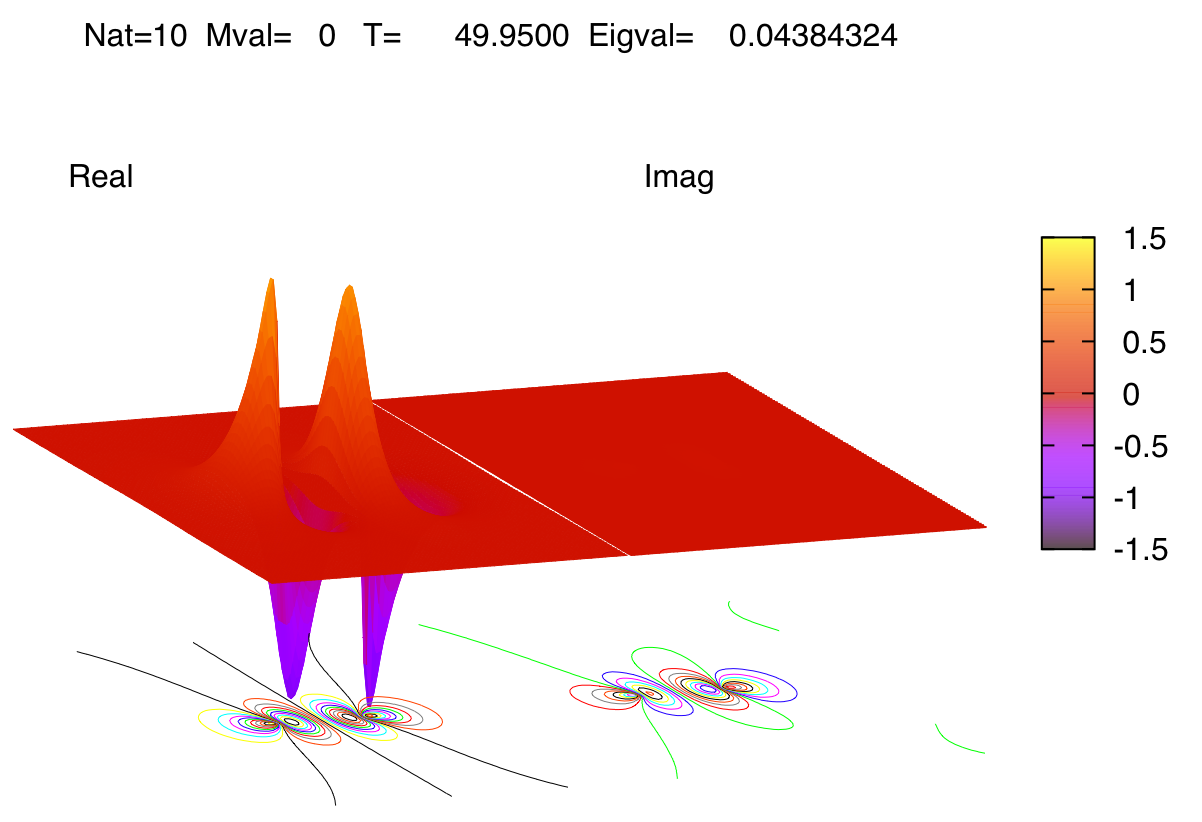
\includegraphics{natplot.png}}
\end{center}
\caption{Example of gnuplot orbital plot.\label{plotfig}}
\end{figure}


\begin{figure}
\begin{center}
\begin{tabular}{ccc}
\resizebox{0.3\columnwidth}{!}{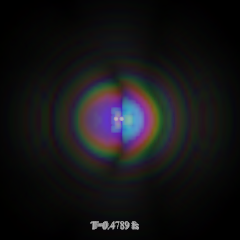
\includegraphics{Spfs_10_T0101_prop1_range2.png}} & 
\resizebox{0.3\columnwidth}{!}{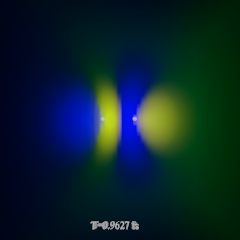
\includegraphics{Spfs_10_T0201_prop1_range1.png}} &
\resizebox{0.3\columnwidth}{!}{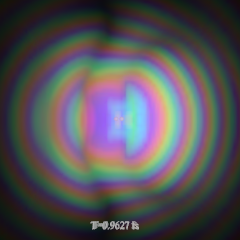
\includegraphics{Spfs_10_T0201_prop1_range2.png}}
\end{tabular}
\end{center}
\caption{Example of Povray natural orbital plot: the tenth ($2\sigma_u$) orbital of a valence-space CAS calculation, directory O2.Small.  Left: at ~0.47 fs, from a range of 40 bond lengths (which are 2.2819... bohr); middle and right, ~0.96fs, from a range of 7 (middle) and 40 (right) bond lengths.  The middle and left plots are the same orbital at the same time.  \label{povplot}}
\end{figure}



Some of the usual output will appear on screen, and then, for instance,
{\small\begin{quote}
\begin{verbatim}
  ****************************** 
     VIEWING NATURAL ORBITALS    
  ****************************** 

USE POVRAY? y for yes.
\end{verbatim}  
\end{quote}}
At this point the plot subroutine branches depending on whether you want to use gnuplot or Povray to produce the output.  Gnuplot may output to screen as either an X11 or AquaTerm plot, or as a .gif file, via the ``change terminal'' option.  Povray produces .tga files which must then be assembled into an animation.  If you answer no to ``USE POVRAY?'' then the following menu will appear for gnuplot:
{\small\begin{quote}
\begin{verbatim}
   What should I do?
          s = change plotskip (now            1 )
          n = change plotnum (now           10 )
          z = change zrange (now    0.8000000000000000      )
          x = change xyrange (now    2.0000000000000000      )
           t = change terminal ( now x11    )
          d = change pm3d (now           0 )
         v1= change view rotation 1 (now    70.000000000000000      ) degrees
          v2= change view rotation 2 (now    70.000000000000000      ) degrees
    default = continue (plot with these options)
c
     Enter natorb number.  Negative to stop.
3
\end{verbatim}
\end{quote}}
If the options are ok you can enter any input except for the labeled options (for instance, type ``c'' then enter) to continue to plot.  Choose the natural orbital or spf that you want to plot.  The program will output some information to screen as it builds the text file for gnuplot.  This may take a while.  Then, a plot should appear, as in Figure \ref{plotfig}.  You then have the option to plot again.

\

If you choose yes to ``USE POVRAY?'' then you will instead only have the following options:
{\small\begin{quote}
\begin{verbatim}
   What should I do?
          s = change plotskip (now            1 )
          n = change plotnum (now           10 )
    default = continue (plot with these options)
\end{verbatim}
\end{quote}}

If you need to change the other parameters for Povray plots, you will need to do this in the input file, in namelist \verb#&parinp#:
{\small\begin{quote}
\begin{verbatim}
&parinp
    povres=14
    numpovranges=2
    povrange=8.0d0, 50.0d0
    povsparse=1.d-3
    ...  /
\end{verbatim}
\end{quote}}
\verb#povres# determines the resolution of the \verb#.df3# file; the data file is $(2 \times $\verb#povres#$ + 1)^3$ big.  \verb#numpovranges# is the number of distances, in units of $R \ a_0$, at which to view the orbitals or density, and the array \verb#povrange# contains those distances.  The parameter \verb#povsparse# determines the zero cutoff for the prolate-to-cartesian transformation matrix -- it is necessary to store this memory in sparse format for large \verb#povres#.  Select an orbital and the plotting subroutine proceeds:
{\small\begin{quote}
\begin{verbatim}
 Enter Natorb     number.  Zero to change options.  Negative to stop.
1
 Good read at record            1
  Maxsparse ... 
   Got maxsparse:           662316                     11523120.
   Got maxsparse:           183544                     11523120.
   Get spherical sparse.
      ...done.
  POV-plotting Natorb !!            0           1   8.0000000000000000     
Persistence of Vision(tm) Ray Tracer Version 3.6.1 (/usr/bin/g++-4.2 4.2.1 @
 i386-apple-darwin10)
\end{verbatim}
\end{quote}}
...and the povray output will continue.  To plot all the natural orbitals or spfs, choose a number of orbitals greater than the number in the calculation.  The program outputs .tga files, which may be assembled by you into an animation.  The output should appear as in Fig.~\ref{povplot}.  The plot is three dimensional and colors the wavefunction according to its phase on the color wheel.  Concentrated parts of the wavefunction may be saturated in what you see.  In Fig.~\ref{povplot}, the middle and left panels are the same orbital at the same time, but at different magnifications; the intensity range is adjusted to different levels according to the magnification of the plot (variable \verb#povranges#). 




\chapter{Examples}

There are several example directories now included in the \verb#EXAMPLES-DEPOT# directory.  As of version 1.16 the following examples
are included:

{\footnotesize
\begin{verbatim}
prompt> ls EXAMPLES-DEPOT/

GAUSSIAN-POTENTIAL-0.13spacing-200pts-scale5-LAWRENCIUM-SCRIPTS
GAUSSIAN-POTENTIAL-0.4spacing-64pts-scale5-LAWRENCIUM-SCRIPTS
H2ABSORPTION-PLAIN-SCRIPTS
H2PHOTO-PLAIN-SCRIPTS
HEPHOTO-PLAIN-SCRIPTS
HELIUM-ATOM-ABSORPTION-PLAIN-SCRIPTS
HELIUM-POLY-ABSORPTION-1.8spacing-45pts-MAC-SCRIPTS
Helium-Neon-ICD-LAWRENCIUM-SCRIPTS
Helium.transient.absorption-bothrotating-weak-LAWRENCIUM-SCRIPTS
Methane.abs.0.39495414.36pts-ion2-MAC-SCRIPTS
Methane.abs.0.39495414.60pts-ion-LAWRENCIUM-SCRIPTS
O2-photo-PLAIN-SCRIPTS
O2-transient-absorption-ONE-PLAIN-SCRIPTS
no2-0.298spacing-49pts-16.22-1x10to16-LAWRENCIUM-SCRIPTS
\end{verbatim}
}

etc.  This chapter goes into these examples.  In the example directories, you will find bash scripts for doing a variety of things.
We imagine that users will adapt these scripts to their needs.  They provide functionality for various things but most notably,
using the method of Domcke et al. [CITE] for calculating macroscopically phase matched signals nonlinear wave mixing experiments.



\section{Total and partial photoionization cross sections: directories H2PHOTO, HEPHOTO, O2-photo }

A total or partial photoionization cross section calculation is performed in four or five steps.  
The same primitive basis should be used for all steps.
%
\begin{itemize}
\item{1) Relaxation for initial state, \verb#Input.Inp.Relax# in the examples}
\item{2) For partial photoionization cross sections, one or more \verb#Input.Inp.Cation#s must be run to produce the $(N-1)$-electron wave functions
that are used for projection.}
\item{3) A short pulse propagation, \verb#Input.Inp.Pulse# in the examples.  At the end of the pulse, very little of the wave function should have 
been absorbed by the complex scaled part of the grid.  Otherwise, it won't be counted as flux.}
\item{4) A long propagation that is used to construct the flux-flux correlation function as per the formalism of Meyer [CITE] and paper XX.  The sharper the features
in the photoionization cross section that are to be resolved, and the longer the real part of the grid is,
the longer the propagation must be.  Useful durations range from 100 to 8000 atomic units (2.5 to 20fs).}
\item{5) The final step is the analysis step.  It is run separate from the propagation. }
\end{itemize}

Again, all the inputs for the \verb#EXAMPLES/# calculations are collected at the end of the chapter.  

\

The \verb#H2PHOTO# and \verb#HEPHOTO# directories are very similar and include scripts for total photoionization. 
\verb#O2-photo# also includes partial photoionization.

The MCTDHF calculation for the photoionization calculation is performed by the following three steps, in order:

 {\footnotesize
 \begin{verbatim}
 prompt> chmctdhf_diatom Inp=Input.Inp.Relax |tee Outs/Out.Relax 
 prompt> chmctdhf_diatom Inp=Input.Inp.Relax |tee Outs/Out.Pulse
 prompt> chmctdhf_diatom Inp=Input.Inp.Fourier |tee Outs/Out.Fourier
 \end{verbatim}
}
While the last is running, one may calculate the cross section so far computed.  A script \verb#Flux.Bat# is included in the example
directories; here is is for \verb#H2PHOTO#: 
 {\footnotesize
 \begin{verbatim}
if [[ "$1 " == " " ]]
then
        echo "need time"
        exit
fi
ee=`grep T= Outs/Out*ax |tail -n 1 |colrm 1 28 |colrm 21 10000 |cut -f 1 -d "E"`
energy=`echo "$ee * 10" |bc -l`
chmctdhf_diatom Inp=Input.Inp.Fourier Act=16   Eground=$energy T=$1 |tee Outs/Out.flux.t$1
cp Dat/xsec.spi.dat Dat/xsec.spi.dat.t$1
\end{verbatim}
}

For \verb#O2-photo#, 
to calculate the cation wave functions for partial photoionization, one can use the script \verb#RunCat.Bat# if working
on a parallel machine (\verb#RunCat.Bat# uses \verb#mpirun# so that killing the \verb#wait# command kills all of them).  This does all of the cation wave functions at once.
Otherwise, run each cation input, e.g. \verb#Input.Inp.Cation.pi_g#, manually, or edit \verb#RunCat.Bat# to your purposes.  Here is \verb#RunCat.Bat#:

{\footnotesize
\begin{verbatim}
 for ext in doub quart; do for sym in sig pi; do for ger in u g
 do 
 mpirun -n 1 chmctdhf_diatom.seq Inp=Input.Inp.Cation.$ext.${sym}_${ger} |tee Outs/Out.cation.$ext.${sym}_${ger} & 
 done; done; done
 wait
\end{verbatim}
}
 



Again, in these examples the \verb#&parinp# namelist input variable 
\verb#eground# is not set in the input, so one must specify it on the command line.
Script \verb#ProjFlux.Bat# in \verb#O2-photo# takes care of this.  Here is the guts of \verb#ProjFlux.Bat#:

{\footnotesize
\begin{verbatim}
if [[ "$2 " == " " ]]
then
        echo "need time and extension"
        exit
fi
rm WALKS/cation.configlist.BIN
rm Bin/cation.spfs.bin Bin/cation.avector.bin
ln -s cation.configlist.BIN.$2 WALKS/cation.configlist.BIN
ln -s avector.bin.cation.$2 Bin/cation.avector.bin
ln -s spfs.bin.cation.$2 Bin/cation.spfs.bin
ee=`grep T= Outs/Out*ax |tail -n 1 |colrm 1 28 |colrm 21 10000 |cut -f 1 -d "E"`
energy=`echo "$ee * 1000" |bc -l`
chmctdhf_diatom Inp=Input.Inp.Fourier Act=17   Eground=$energy T=$1 |tee Outs/Out.projflux.t$1
for file in Dat/FTGTau*_*Dat Dat/KVLsum*_*dat Dat/xsec.proj*_*dat
do
        mv $file $file.$2
done
\end{verbatim}
}
For O$_2$ partial photoionization there are many final cation states with different symmetries.  
However currently the projected flux can only be calculated
for one set of cation states at a time.  Always, it needs \verb#WALKS/cation.configlist.BIN#, the cation 
configuration list, and the cation wave function(s), \verb#Bin/cation.spfs.bin# and \verb#cation.avector.bin#.
These file names are hard wired in the code presently.  
In the input files that are run by \verb#RunCat.Bat#, the output file names are specified, for instance,
{\footnotesize
\begin{verbatim}
configlistfile="WALKS/cation.configlist.BIN.doub.pi_g"
avectoroutfile="Bin/avector.bin.cation.doub.pi_g"
spfoutfile="Bin/spfs.bin.cation.doub.pi_g"
\end{verbatim}
}
and so, as you can see above, what \verb#ProjFlux.Bat# does is make symbolic links to these files.


\section{H2ABSORPTION, HE-ATOM-ABSORPTION directories (action 21, absorption/emission, Fourier transform dipole moment)}


XXXX

XXXX

XXXX



\section{Benzene}

\section{Diels-Alder}

\section{Helium-Neon Interatomic Coulombic Decay}

\section{Transient absorption/emission and wave mixing}

The code calculates the expectation value of the dipole moment and fourier transforms it using action 21.  The output can be post
processed.  The example directory
\verb#Helium.transient absorption#
is included in the \verb#EXAMPLES# subdirectory.  

\subsection{O2.transient.absorption.ONE}

\subsection{2D spectra for O$_2$ and He}



\chapter{Programmers' guide}


Again, the directory structure, right out of the package, is as follows. 

{\footnotesize
\begin{verbatim}
   MCTDH.SRC
      DFFTPACK
      DGMRES
      SINCDVR
      H2PROJECT
      HEPROJECT
   COMPDIRS
      MCTDH.SRC -> ../MCTDH.SRC
      BIN.ecs.hermnorm.law.openmp.nofft
         Definitions.INC
         Name.Txt
         Makefile.header -> ../MCTDH.SRC/Makefile.header.lawrencium.openmp.nointelfft
         Definitions.ALL -> ../MCTDH.SRC/Definitions.ALL
         mctdhf.F90 -> ../MCTDH.SRC/mctdhf.f90
         DFFTPACK
            Makefile.header -> ../Makefile.header
            Makefile -> ../../MCTDH.SRC/DFFTPACK/Makefile
            zfftf1.f -> ../../MCTDH.SRC/DFFTPACK/zfftf1.f
         SINCDVR
            Makefile.header -> ../Makefile.header
            Makefile -> ../../MCTDH.SRC/SINCDVR/Makefile
            sincDVR.f90 -> ../../MCTDH.SRC/SINCDVR/sincDVR.f90
      debug.BIN.ecs.hermnorm.mac
      BIN.mac
      BIN.ecs.hermnorm.edison
\end{verbatim}}

Notice the following things.
\begin{itemize}
\item{The \verb#*BIN*# compilation directories are identical 
except for \verb#Name.txt#, \verb#Makefile.header#, and \verb#Definitions.INC#.}
\item{All of the subdirectories of these \verb#BIN# directories are real subdirectories; they contain nothing but links.}
\item{Notice that most of the symbolic links to fortran files end in \verb#.F90# whereas all the fortran files themselves
in \verb#MCTDH.SRC# end in \verb#.f90#.  This is done to invoke the c preprocessor with some compilers (with the
\verb#.F90#) but the fortran interpreter with emacs (with the \verb#.f90#).}
\item{The compilation directories have
Symbolic links and directory-specific 
 \verb#Name.txt#, \verb#Makefile.header#, and \verb#Definitions.INC#.}
\end{itemize}


These \verb#BIN# directories contain the compiled version of the code and all the object files and miscellaneous files created
during compilation.
They have subdirectories, symbolic links, and two real files, \verb#Definitions.INC# and \verb#Name.Txt#:


%
\verb#Name.Txt# contains the name of the program version, e.g. \verb#chmcdthf# for \verb#chmctdhf_diatom#, etc.;  
alternatively
\verb#mctdhf#, \verb#pmctdhf#, or \verb#cmctdhf#; and is used by the Makefile.
\verb#Definitions.INC# is a header for most of the \verb#.f90# files that contains preprocesor directives that define data 
types and the corresponding LAPACK subroutines differently for the different BIN directories, implementing real or 
complex data types, ECS or no ECS, and hermitian norm or, for ECS, c-norm, \verb#mctdhf#, \verb#chmctdhf#,
\verb#pmctdhf#, \verb#cmctdhf#.  To effect the differences, the macros \verb#REALGO#, 
\verb#ECSFLAG#, and \verb#CNORMFLAG# are either defined or undefined, and then there are conditional statements 
that do the rest of the work in \verb#Definitions.ALL#.

\

\verb#Definitions.INC# \ {\bf :}

{\small
\begin{quote}
\begin{verbatim}
#define REALGO
#define ExxCSFLAG
#define CxxNORMFLAG

#include "Definitions.ALL"
\end{verbatim}
\end{quote}}

\verb#Definitions.ALL# \ {\bf :}

{\small
\begin{quote}
\begin{verbatim}
#ifdef REALGO

#define DATATYPE real*8
#define MYGEMM DGEMM
...
\end{verbatim}
\end{quote}}
The fortran files then use these c preprocessor macros,
{\small
\begin{quote}
\begin{verbatim}
#include "Definitions.INC"

module automod
  implicit none

  DATATYPE, allocatable :: overlaps(:,:)
  integer, allocatable :: calledflags(:)
...
\end{verbatim}
\end{quote}}

\section{Main program files}

The \verb#MCTDH.SRC# directory contains the following files.  They are grouped by nature and importance.
\verb#parameters.f90# and \verb#main_modules.f90# are the main dependencies; most of the other files depend
on these files, and none other.  Again we reiterate that we sometime use the terms configuration and slater determinant 
interchangeably.  Sometimes when we write configuration, we mean either a slater determinant or a spin adapted sum
of slater determinants.  But usually, we just mean slater determinant.

{\footnotesize
\begin{verbatim}

-rw-------  Definitions.ALL                 x C preprocessor macros
-rw-------  Makefile.header.edison          x Makefile.headers
-rw-------  Makefile.header.mac.mpi.debug   x   . . . etc
-rw-------  Makefile                        x Makefile
-rwxr-xr-x  Makeme                          x Compilation script

drwx------  DFFTPACK                        x Fourier transform
drwx------  DGMRES                          x GMRES
drwxr-xr-x  COREPROJECT                     x coreproject.f90
drwx------  HEPROJECT                       x Atom project
drwx------  H2PROJECT                       x Diatom project

-rw-------  parameters.f90                  x VARIABLES, Namelist &parinp
-rw-------  main_modules.f90                x Modules
-rw-------  getparams.f90                   x Routine to load input file, otherwise set variables

-rw-------  mctdhf.f90                      x Main program
-rw-------  prop.f90                        x Core of main program
-rw-------  derivs.f90                      x Orbital propagation subroutines - working equation, call of expo_driver
-rw-r--r--  configstuff.f90                 x Subroutine for configuration propagation and diagonalization

-rw-------  expo_driver.f90                 x Orbital propagation subroutines - call of expokit

-rw-------  matel.f90                       x Orbital and configuration matrix element subroutines

-rw-------  mean.f90                        x Constructs 2-e reduced denmat
-rw-------  denmat.f90                      x 1-e reduced denmat and miscellaneous (denmat constraint for restricted
                                                                             configuration list)
-rw-------  walks.f90                       x Matrix elements among slater determinants
-rw-r--r--  walkmult.f90                    x Use them to multiply vector of configuration coefficients
-rw-r--r--  newconfig.f90                   x Configuration subroutines (get configuration list, get configuration index)
-rw-------  spin.f90                        x Spin (S(S+1)) adaptation
-rw-------  spinwalks.f90                   x Matrix elements of spin operator among configurations

-rw-r--r--  biortho.f90                     x Biorthogonalization workhorse

-rw-r--r--  driving.f90                     x Psi-prime treatment

-rw-------  quad.f90                        x Improvedquadflag - inverse iterations for diagonalization

-rw-------  second_derivs.f90               x Verlet intopt=4

-rw-r--r--  blocklanczos.f90                x Diagonalization

-rw-------  dfconstrain.f90                 x Restricted configuration list - computation of g and tau, orbital derivatives

-rw-------  actions.f90                     x Action driver routines.
-rw-------  autocall.f90
-rw-------  autosub.f90
-rw-------  readactions.f90
-rw-r--r--  saveactions.f90
-rw-r--r--  natprojaction.f90
-rw-------  povactions.f90
-rw-r--r--  orbvectoractions.f90
-rw-r--r--  dipolecall.f90
-rw-------  dipolesub.f90
-rw-------  electronflux.f90
-rw-------  projeflux.f90
-rw-------  ovlsub.f90
-rw-r--r--  keprojector.f90

-rw-------  MPI.f90                         x Parallel subroutines
-rw-r--r--  proputils.f90                   x Utilities, including pulse subroutines
-rw-r--r--  spfs.f90                        x Utilities relating to orbitals
-rw-------  eigen.f90                       x LAPACK wrappers
-rw-r--r--  utils.f90                       x Miscellaneous
-rw-r--r--  psistats.f90                    x Expectation values of wave function
-rw-r--r--  configload.f90                  x I/O
-rw-r--r--  loadstuff.f90                   x I/O

-rw-------  expokit.f                       x Exponential propagator for orbitals, also psi-prime & miscellaneous 
                                                   Roger B. Sidje U Queensland         modified in key places by me
-rw-------  gaussq.f                        x Quadrature
-rw-------  jacobi.f                        x Quadrature
-rw-------  odex.f                          x Implicit integrator intopt=1
-rw-------  opkda1.f                        x General purpose solver intopt=2
-rw-------  rkf45.f                         x Runge-Kutta intopt=0
-rw-------  arg.c                           x Some c routines
\end{verbatim}
}

\section{Project directories}

The project directories contain files required to build the different compiled versions of the code, running different coordinate systems.  In the past,
the code had a flag, and all coordinate systems were contained in one program; now it is different.

There are three projects currently, atom, diatom, and polyatomic,
in \verb#H2PROJECT#, \verb#HEPROJECT#, and \verb#SINCPROJECT#, respectively.  The first two share one file; duplication is avoided by
 writing one file, \verb#MCTDH.SRC/COREPROJECT/coreproject.f90#,
that is shared.  This is not the general operation; project directories, like \verb#SINCPROJECT#, in general should be autonomous.  

To add a new project directory, put the source code in a subdirectory of \verb#MCTDH.SRC#, perhaps \verb#MCTDH.SRC/NEWPROJECT#; 
then create a directory (not a link, \verb#mkdir#) in one of the \verb#BIN# directories, also called \verb#NEWPROJECT#.  Then, go into that directory and
link each the files in \verb#MCTDH.SRC/NEWPROJECT# to \verb#BIN/NEWPROJECT#, with the same name except for capital-F \verb#.F90# extension.

That should set up \verb#BIN/NEWPROJECT#; then you can recursively copy \verb#BIN.NEWPROJECT# to \verb#BIN.ecs.hernorm.debug# or any
other compilation directories that you have set up (keeping symbolic links as symbolic links!!) and they should be ready to go, if you did your \verb#Makefile# in \verb#NEWPROJECT# like
it is in the existing project directories.

\section{About the Makefile and Makeme}

The code is meant to be compiled with the script \verb#Makeme# which should be linked in the \verb#BIN# directory in question.  All it does
is run \verb#make# in the project directories, the other subdirectories, and then in the main directory.  So if one adds a project, one adds a line
in \verb#Makeme#, to compile the code in the project directory that you have designed (with your makefile, which should be invoked by the
``\verb#make#'' command that \verb#Makeme# runs in your project directory).  
In the \verb#Makefile#, one would add a new project called ``newproject'' as follows.
\begin{verbatim}
MYDEFAULT=$(NAME)_atom $(NAME)_diatom $(NAME)_sinc $(NAME)_newproject

NEWPROJECT=NEWPROJECT/myprojectar.a
HEPROJECT=HEPROJECT/heprojectar.a
H2PROJECT=...
\end{verbatim}
and an instruction lower down,
\begin{verbatim}
$(NAME)_newproject:   $(SRCS) mctdhf.o  $(NEWPROJECT)
        $(F90) $(LOADFLAGS) -o $(NAME)_newproject  $(openmp) $(DFFTPACK) $(SRCS) mctdhf\
.o $(bessrcso) $(DFFTFILES) $(dgmfiles) $(dgmparfiles) $(NEWPROJECT) ...
\end{verbatim}

The makefile starts out by including the file \verb#Makefile.header# 
which has your compiler options, and also the file \verb#Name.txt# which just has the name of the code for the particular \verb#BIN# directory.  For instance, for \verb#BIN.ecs.hermnorm#,
\verb#Name.txt# is as follows:
\begin{quote}
\verb#NAME=chmctdhf#
\end{quote}


\section{Important variables}


It's all about the \verb#xarr# data type and the variable \verb#yyy#.  But also you need to understand how the sparse matrix routines are done --
data types \verb#Type(CONFIGPTR)# and \verb#Type(SPARSEPTR)#.


The key variables are \\

\verb#yyy# 
\begin{quote}
 yyy is type \verb#xarr# that \verb#actions.f90# and \verb#prop.f90# some other things can use via \verb#xxxmod#.  It contains the
 wave function and other things, for the current time step (time step 0) and the previous one (time step 1).
\end{quote}

\verb#yyy%cmfpsivec(:,0)#
\begin{quote}
The wave function (orbital coefficients and A-vector) at the present time step.  yyy\%cmfpsivec(:,1) is the one previous.
\end{quote}

\verb#spfstart, astart(mcscfnum)# 
\begin{quote}
For \verb#psitype=1#, a CI wavefunction, these are the indices at which the 
SPF-vector and A-vector start.  Thus, to pass a subroutine the current spfs, use 
 \verb#call mysub(yyy%cmfpsivec(spfstart,0))#.
\end{quote}
 
\verb#spftotdim# 
\begin{quote}
 This is the size of the SPF-vector. 
\end{quote}
 
\verb#totadim# 
\begin{quote}
 This is the size of the A-vector. 
\end{quote}
 
 ...not finished
 
 \section{Project directories}
 \subsection{Functions/subroutines that are necessary to define}
 
\end{document}





